\documentclass[draft,swe,10pt,nofont]{skrapport}
%% Packages (fold)
% Packages included by <skrapport>:
% polyglossia, microtype, icomma, amsmath,
% unicode-math, xunicode, fontspec
% graphics
\usepackage[usenames,dvipsnames]{xcolor}
\usepackage{graphicx}
\usepackage{tikz}
\usetikzlibrary{shadows}
% page size
\usepackage[c5paper,xetex]{geometry}
% code
\usepackage{minted}
% improvement packages
\usepackage{multirow}
\usepackage[hyperfootnotes=false,colorlinks=true,linkcolor=Red,urlcolor=Magenta]{hyperref}
\usepackage[swedish]{varioref}
\usepackage[para,perpage,ragged,bottom,stable]{footmisc}
\usepackage{enumitem}
\usepackage{fancyhdr}
\usepackage{booktabs}
% references
\usepackage[swedish]{chscite}
% other stuff
\usepackage{ifdraft}
\usepackage{siunitx}
\usepackage{hologo}
\usepackage[safe,noenc]{tipa}
\usepackage[titles]{tocloft}
\usepackage{titlesec}
\usepackage[font=small,format=plain,labelfont=bf,textfont=it]{caption}
\usepackage{subfig}
\usepackage{sidecap}
\usepackage{cprotect}
\usepackage{bookmark}
\usepackage{xspace}
\usepackage{mathtools}
% Source code line numbers in margin
\usepackage{srcline}
% Paket som demonstreras i del 6
\usepackage{braket}
\usepackage{amscd}
\DeclareMathOperator\add{add}
\DeclareMathOperator\cov{cov}
\DeclareMathOperator\non{non}
\DeclareMathOperator\cf{cf}
%% (end)

%% Draft fixes to minted, tikz (fold)
\ifdraft{%
\renewcommand\mint[3][]{\DefineShortVerb{#3}\fvset{#1}\SaveVerb[aftersave={\UndefineShortVerb{#3}\begin{flushleft}\UseVerb{minted@verb}\end{flushleft}}]{minted@verb}#3}%
\renewenvironment{minted}[2][]{\VerbatimEnvironment\fvset{#1}\begin{Verbatim}}{\end{Verbatim}}
\renewcommand\inputminted[3][]{\fvset{#1}\VerbatimInput{#3}}
% LaTeX source code
\newminted{latex}{frame=single}%
\newminted{text}{frame=single}%
\newmint{latex}{frame=single}%
% Line numbers in margin
\lnoson% % Disable when not spellchecking/proofreading
}{%
% LaTeX source code
\newminted{latex}{frame=single,bgcolor=mintedbg,rulecolor=\color{mintedbg}}%
\newminted{text}{frame=single,bgcolor=mintedbg,rulecolor=\color{mintedbg}}%
\newmint{latex}{frame=single,bgcolor=mintedbg,rulecolor=\color{mintedbg}}%
}
%% (end)

%% FONT SELECTION (fold)
\defaultfontfeatures{%
	Numbers={Proportional,OldStyle},%
	Ligatures={Historic,Common,Required,Contextual},%
	Contextuals=Swash,%
	SmallCapsFeatures={Letters=SmallCaps,Scale=0.96,Weight=0.8},%
}
\setmainfont[Scale=1.1,SmallCapsFont={ArnhemSmallCaps}]{Baskerville}
\setsansfont[Scale=0.935]{Frutiger LT Std}
\setmonofont[Scale=0.935]{Prestige Elite Std}
\newfontfamily\titlefont[%
	Alternate=0,%
	%Ligatures={Rare,Historic,Common,Required,Contextual}%
]{Hoefler Text}
\newfontfamily\utffont{Times New Roman}% Change this?
\newfontfamily\tipafont{DejaVu Serif}
%\setmathrm{Asana Math}
%\setmathsf{}
%\setmathtt{}
%\setboldmathrm{}
\makeatletter\newcommand\@titstyle{\titlefont}\makeatother
%% (end)

%% Hacks (fold)
\makeatletter
% Fix \hologo{XeTeX}
\def\HoLogo@Xe#1{% 
   X% 
   \kern-.1em\relax 
   \ltx@IfUndefined{HOLOGO@ReflectBox\hologodriver} 
     {\ltx@IfUndefined{HOLOGO@ReflectBox}\ltx@firstoftwo\ltx@secondoftwo} 
     \ltx@secondoftwo 
   {e}{% 
     \lower.5ex\hbox{% 
       \HOLOGO@ReflectBox{E}% 
     }% 
   }% 
}
% Force cramped style on inline math
\def\(#1\){\relax\ifmmode\@badmath\else$\fi\cramped{#1}\relax\ifmmode\ifinner $\else\@badmath\fi\else\@badmath\fi}
%\def\(#1\){\relax\ifmmode\@badmath\else$\fi\smash{#1}\relax\ifmmode\ifinner $\else\@badmath\fi\else\@badmath\fi}
% Varioref seems broken with XeLaTeX
\def\reftextfaceafter{på \reftextvario{motstående}{nästa} sida}%
\def\reftextfacebefore{på \reftextvario{motstående}{föregående} sida}%
\def\reftextafter{på \reftextvario{följande}{nästa} sida}%
\def\reftextbefore{på föregående sida}%
\def\reftextcurrent{på denna sida}%
\def\reftextfaraway#1{{på sidan~\pageref{#1}}}%
\def\reftextpagerange#1#2{{på sidorna~\pageref{#1}–\pageref{#2}}}%
\def\reftextlabelrange#1#2{{\ref{#1} till~\ref{#2}}}%
\DeclareRobustCommand\Vref{\@ifstar{\let\vref@space\relax\Vr@f}{\let\vref@space~\Vr@f}}
\DeclareRobustCommand\vref{\@ifstar{\let\vref@space\relax\vr@f}{\let\vref@space~\vr@f}}
% Twoside
\@twosidetrue
% Listings
\newcommand{\kodname}{Exempel}
\newcounter{kod}\renewcommand\thekod{\@arabic\c@kod}
\def\fps@kod{tb}
\def\ftype@kod{3}
\def\ext@kod{lok}
\def\fnum@kod{\kodname~\thekod}
\newenvironment{kod}{\@float{kod}}{\end@float}
\newenvironment{kod*}{\@dblfloat{kod}}{\end@dblfloat}
\newsubfloat{kod}
% Displaying one line of code
\newcommand\kodrad[2]{\hspace{1ex}\inputminted[firstline=#1,lastline=#1]{latex}{#2.tex}}
% Redefining sections to break page
\let\section@old=\section
\renewcommand\section{\@ifstar\my@section@star\my@section}
\newcommand\my@section[2][\@empty]{\cleardoublepage\vspace*{2\bigskipamount}\ifx\@empty#1\section@old{#2}\else\section@old[#1]{#2}\fi}
\newcommand\my@section@star[2][\@empty]{\cleardoublepage\vspace*{2\bigskipamount}\ifx\@empty#1\section@old*{#2}\else\section@old*[#1]{#2}\fi}
% Front/main/backmatter
\newcommand\frontmatter{%
  \cleardoublepage
  \pagenumbering{roman}}
\newcommand\mainmatter{%
  \cleardoublepage
  \pagenumbering{arabic}}
\newcommand\backmatter{%
  \cleardoublepage
}
% Maketitle without newpage
\newcommand\maketitlennp{\par%
  \begingroup
    \renewcommand\thefootnote{\@fnsymbol\c@footnote}%
    \def\@makefnmark{\rlap{\@textsuperscript{\normalfont\@thefnmark}}}%
    \long\def\@makefntext##1{\parindent 1em\noindent%
      \hb@xt@1.8em{\hss\@textsuperscript{\normalfont\@thefnmark}}##1}%
    \global\@topnum\z@
    \@maketitlennp
    \thispagestyle{empty}\@thanks
  \endgroup
  \setcounter{footnote}{0}
}
\def\@maketitlennp{%
  \null
  \begin{flushleft}%
\vspace{-\headsep}
    {\small%
      \if\@regarding\relax\else\@regarding{, }\fi%
      \@date\par%
    }%
    \vspace{1.5cm}%
    {\Huge\@titstyle\@title\par}%
    \vspace{.125cm}%
    {\Large\@titstyle\@author}%
    \vspace{.75cm}%
  \end{flushleft}%
  \par%
}
% Changes to titlepage environment (don't reset pagenumbering before)
\renewenvironment{titlepage}{\cleardoublepage}{\thispagestyle{skrapport@titlepage}\cleardoublepage\setcounter{page}\@ne}
% TexorPDF version of LaTeX and AmS logo
\let\@oldLaTeX\LaTeX
\def\LaTeX{\texorpdfstring{\@oldLaTeX}{LaTeX}}
\let\@oldAmS\AmS
\def\AmS{\texorpdfstring{\@oldAmS}{AMS}}
% File last modified
\def\parsedate #1:2#2#3#4#5#6#7#8#9\empty{\ifx{#2}{9}19\else20\fi#3#4/#5#6/#7#8}
\newcommand\moddate[1][\jobname.tex]{\expandafter\parsedate\pdffilemoddate{#1}\empty}
% Minted background fix
\renewenvironment{minted@colorbg}[1]{%
	\par%
	\def\minted@bgcol{#1}%
	\noindent\begin{lrbox}{\minted@bgbox}%
	\begin{minipage}{\linewidth-2\fboxsep}%
}{%
	\end{minipage}%
	\end{lrbox}%
	\colorbox{\minted@bgcol}{\usebox{\minted@bgbox}}%
	\par%
}
\makeatother
% (end)

%% Convenient definitions (fold)
\newcommand\PDF{\textsc{PDF}\xspace}					% PDF format
\newcommand\DVI{\textsc{DVI}\xspace}					% DVI format
\newcommand\EPS{\textsc{EPS}\xspace}					% EPS format
\newcommand\UTF{\textsc{UTF-8}\xspace}					% UTF-8 standard
\newcommand\cli[1]{\texttt{#1}}							% Command-line input
\newcommand\opt[1]{\texttt{\emph{#1}}}					% CLI option
\newcommand\pack[1]{\textsf{#1}}						% LaTeX package
\newcommand\pdfLaTeX{\hologo{pdfLaTeX}\xspace}			% pdfLaTeX logotype
\newcommand\BibTeX{\textsc{Bib}\TeX\xspace}				% BibTeX logotype
\newcommand\PGFTikZ{PGF/Ti\emph{k}Z\xspace}				% PGF/TikZ logotype
\newcommand\XeTeX{\hologo{XeTeX}\xspace}				% XeTeX logotype
\newcommand\LyX{L\!\raisebox{-.5ex}{Y}\!X\xspace}		% LyX logotype
\newcommand\eng[1]{(eng.~\textenglish{\emph{#1})}}		% english translation
\newcommand\cmd[1]{\textenglish{\texttt{\textbackslash{}#1}}}% LaTeX command
\newcommand\env[1]{\textenglish{\texttt{#1}}}			% LaTeX environment
% Front/back page color and graphics
\def\frontpagecolor{LimeGreen}
\newcommand\frontpagegraphic{\begin{tikzpicture}[remember picture,overlay]
	\coordinate [below=2.225cm] (midpoint)
					   at (current page.north);
	\node [anchor=north,fill=Black,opacity=0.25,
	minimum width=\paperwidth,
	minimum height=6cm] at (midpoint) {};
\end{tikzpicture}}
% minted style
\usemintedstyle{solarized}
\definecolor{mintedbg}{rgb}{0.9665,0.9550,0.9175}
% Unit definitions
\DeclareSIUnit\point{pt}
\DeclareSIUnit\em{em}
\DeclareSIUnit\mu{mu}
\sisetup{locale=DE}
% Math redefinitions
\DeclareMathOperator{\erfc}{erfc}
\renewcommand{\frac}[2]{\genfrac{}{}{}{}{\displaystyle #1}{\displaystyle #2}}
\makeatletter
\renewcommand\d[1]{\ensuremath{\,\mathrm{d}#1\@ifnextchar\d{\!}{}}}
\makeatother
% Useful colors
\definecolor{required}{rgb}{0.384,0.576,0.000}
\definecolor{optional}{rgb}{0.992,0.843,0.000}
\definecolor{unavailable}{rgb}{0.863,0.196,0.184}
%% (end)

%% Redefinitions of style (fold)
\setcounter{secnumdepth}{1}				% Section numbering depth
\setcounter{tocdepth}{2}				% Table of contents depth
\renewcommand{\cftsecfont}{\bfseries}	% Table of contents bf sections
\fancypagestyle{thefancy}{%
	\fancyhead{}
	\fancyfoot{}
	\fancyhead[LE,RO]{\thepage}
	\renewcommand{\headrulewidth}{0.1pt}
}
\headheight 15pt
\makeatletter
\renewcommand\thesection{\Roman{section}}
\titleformat{\section}[block]{\centering\Huge\@titstyle}{\makebox[\textwidth]{\fontsize{36pt}{36pt}\selectfont\centering\thesection}}{0pt}{\newline}[\bigskip]
% Holy shit, hacking my own class
\let\c@paragraph\relax\let\c@subparagraph\relax 
\let\paragraph\relax\let\subparagraph\relax
\newcommand\subsubsubsection{\@startsection{subsubsubsection}{4}{\z@}%
  {-2ex \@plus .5ex \@minus -.5ex}%
  {.125ex \@plus.125ex}%
  {\normalfont\large\@titstyle\itshape}}
\newcommand\paragraph{\@startsection{paragraph}{5}{\z@}%
  {1ex \@plus .25ex \@minus -.25ex}%
  {-1em}%
  {\normalfont\normalsize\bfseries}}
\newcommand\subparagraph{\@startsection{subparagraph}{6}{\parindent}%
  {1ex \@plus .25ex \@minus -.25ex}%
  {-1em}%
  {\normalfont\normalsize\itshape}}
\newlistentry[subsubsection]{subsubsubsection}{toc}{3}
\newlistentry[subsubsubsection]{paragraph}{toc}{4}
\newlistentry[paragraph]{subparagraph}{toc}{5}
\cftsetindents{subsubsubsection}{6.45em}{4.15em}
\cftsetindents{paragraph}{10.6em}{5.15em}
\cftsetindents{subparagraph}{15.75em}{6.15em}
\providecommand*{\toclevel@subsubsubsection}{4}
\providecommand*{\toclevel@paragraph}{5}
\providecommand*{\toclevel@subparagraph}{6}
\renewcommand\thesubsubsubsection{\thesubsubsection.\@arabic\c@subsubsubsection}
\renewcommand\theparagraph{\thesubsubsubsection.\@arabic\c@paragraph}
\renewcommand\thesubparagraph{\theparagraph.\@arabic\c@subparagraph}
\makeatother
%% (end)

%% METADATA (fold)
\title{Att \TeX{}a: en praktisk guide}
\author{Simon Sigurdhsson}
\regarding{Nybörjarguide i \LaTeX}
\date{första upplagan.}
%% (end)

\begin{document}
	\pagestyle{empty}
	\pagenumbering{Alph}
	
	{ % EXTERNAL FRONT PAGE (fold)
		\pagecolor{\frontpagecolor}
		\color{White}
		\frontpagegraphic
		\maketitlennp		
		\normalcolor
		\newpage
		\pagecolor{White}
	} % (end)
	\cleardoublepage
	
	\begin{titlepage} % INTERNAL TITLE PAGE (fold)
		\license{%Senast uppdaterad \moddate{}.\\
		Licenserad under Creative Commons By-Nc-Nd-2.5.\\
		\url{http://creativecommons.org/licenses/by-nc-nd/2.5/se/}\\
		För användning utanför licensen, kontakta författaren.}
		\maketitle
		\begin{abstract}
			En inkomplett guide till att skriva och typsätta \LaTeX-dokument riktad
			till studenter på Chalmers Tekniska Högskola, specifikt programmen
			Teknisk Matematik och Teknisk Fysik.
			Inspiration har tagits från bland annat \citeasnoun{Schultz05} och
			\citeasnoun{Voss10}, men främst från \citeasnoun{Oetiker11}.
		\end{abstract}
	\end{titlepage} % (end)
	\cleardoublepage
	
	\begin{center} % DEDICATION, THANKS AND PUBLISHER
		\large\vspace*{36pt}
		{\makeatletter\@titstyle\makeatother\huge Tillägnad}\\[1ex]
		min underbara flickvän.
		\bigskip\bigskip\bigskip
		
		{\makeatletter\@titstyle\makeatother\Large Tack till}\\[1ex]
		\emph{Phaddergrupp 255},\\
		som korrekturläst och\\
		hjälpt till att förbättra boken\\[1ex]
		{\makeatletter\@titstyle\makeatother\Large och}\\[1ex]
		\emph{Christian von Schultz},\\
		\emph{Tobias Oetiker} och \emph{Herbert Voß}\\
		för inspirerande texter på samma tema.
		\vfill 
		
		\small
		%Tryck: XXX\\
		Göteborg, 2011
	\end{center}
	\cleardoublepage 
	
	\frontmatter
	\pagestyle{thefancy}
	\tableofcontents
	\cleardoublepage
	
	\mainmatter
	%% INLEDNING (fold)
	\section*{Inledning}
	\addcontentsline{toc}{section}{\hspace{1.3em}Inledning}
	Att publicera något, oavsett om det är långa böcker eller korta artiklar,
	är inte helt enkelt. Förr, innan det fanns en dator i varje hem och innan
	programvaror som Microsoft Word och OpenOffice blev tillgängliga för var
	man så var publicering något komplext, något som utfördes av många olika
	personer. Arbetet delades upp i olika bitar och en expert inom varje
	område fick sköta den biten; författande, typsättning, design och så
	vidare.
	
	Moderna programvaror (ordbehandlare, främst) fungerar på ett helt annat
	sätt. De ger all makt till författaren, som givetvis inte alltid är
	särskilt bra på det där med typsättning eller design. Som en konsekvens
	blir typsättningen av dokument inte alltid bra — användarna är under
	illusionen att ett estetiskt tilltalande dokument även är ett bra dokument
	rent typografiskt. Så är givetvis inte fallet.
	
	För att få snygga dokument måste man återskapa den gamla ordningen då
	varje uppgift löstes av någon som var bra på det. En författare ska inte
	behöva berätta \emph{hur} saker ska se ut — det ska designern göra —
	författaren ska bara berätta \emph{vad} saker är\footnote{Detta är inte
	helt olikt den uppdelning som görs mellan HTML och CSS.}. \LaTeX{} låter
	dig som författare göra just detta.
	
	\subsection*{Vad är \LaTeX{}?}
	\addcontentsline{toc}{subsection}{Vad är \LaTeX{}?}
	\LaTeX{} (uttalas \textipa{\tipafont[\textprimstress lA:tEx]}) är i princip en
	påbyggnad till \TeX{}, ett typsättningssystem. Man kan även se det som att
	\LaTeX{} är designern, och \TeX{} är typsättaren. \LaTeX{} berättar i
	någon mening för \TeX{} hur den tror att du vill ha ditt dokument (utifrån
	dokumentklassen samt den kod du skriver) och låter sedan \TeX{} typsätta
	detta för att skapa ett ”tryckt” dokument.
	
	Men \LaTeX{} är inte bara ett typsättningssystem; både språket dokumenten
	skrivs i och den kompilator som omvandlar dokumenten till \DVI-filer
	kallas också \LaTeX{} (men just kompilatorn brukar benämnas \cli{latex},
	eftersom det är så den körs från terminalen). Det finns även modernare
	versioner av \LaTeX{}-kompilatorn, till exempel \pdfLaTeX{} som skapar
	\PDF-dokument
	 direkt (så att man slipper konvertera dem med \cli{dvipdf}) och
	\XeTeX{}, som baseras helt på \textsc{Unicode} och har bättre stöd för
	diverse typsnitt.
	
	\subsection*{Varför \LaTeX?}
	\addcontentsline{toc}{subsection}{Varför \LaTeX{}?}
	Fördelen med \LaTeX{} är då att författaren endast behöver lära sig några
	enkla kommandon — sådana som gör texten kursiv eller infogar en figur
	— men att dokumentet ändå håller mycket hög standard, precis som om
	det typsatts av en riktig typsättare.
	
	Eftersom språket man skriver dokument i uppmanar till struktur och ordning
	blir det dessutom lättare att skriva strukturerade texter. Även om saker
	som finns i en vanlig ordbehandlare (stavningskontroll, till exempel) saknas i
	själva språket så kan (och bör) dessa tillhandahållas av externa program,
	vilket gör att \LaTeX{} kan koncentreras på att vara bra på \emph{en} sak:
	att typsätta dokument. Saker som är komplicerade eller omöjliga att göra
	i en vanlig ordbehandlare, till exempel korsreferenser, figurer, tabeller,
	fotnoter, referenslistor och dylikt är oerhört enkla att göra i \LaTeX{}
	och oftast fullt automatiserade.
	
	Dessutom har \LaTeX{} traditionellt använts av akademiker eftersom det gör 
	typsättning av just matematik och fysik både enkel och visuellt attraktiv. 
	
	\subsection*{I denna introduktion}
	\addcontentsline{toc}{subsection}{I denna introduktion}
	Den här korta introduktionen kommer att visa dig hur man på ett enkelt
	sätt typsätter dokument med \LaTeX{} i vanliga tillämpningar.
	Dessutom kommer den framåt slutet peka på specifika paket eller
	resurser som kan vara användbara för mer avancerade fall.
	
	Efter att ha läst den här introduktionen bör läsaren kunna skriva
	dokument och rapporter utan problem. Det är dock inte tänkt att denna
	introduktion ska vara en fullgod referens till \LaTeX; för detta
	rekommenderas istället \citeasnoun{Lamport94} och
	\citeasnoun{Mittelbach04}.
	
	Introduktionen innehåller följande delar:
	\begin{description}
		\item[{Del \ref{sec:1}, \hyperref[sec:1]{Grundläggande begrepp}}]
		beskriver den grundläggande strukturen hos \LaTeX-dokument och hur det
		språk dokumenten skrivs i fungerar i korta drag. Efter denna del bör
		du veta på ett ungefär hur \LaTeX{} fungerar.
		
		\item[{Del \ref{sec:2}, \hyperref[sec:2]{Typsättning med \pdfLaTeX}}]
		beskriver i detalj hur man skriver ett vanligt
		\LaTeX-dokument, och förklarar några av de viktigaste miljöerna
		och kommandona som används. Efter denna del bör du kunna skriva enkla
		dokument med \LaTeX.
		
		\item[{Del \ref{sec:3}, \hyperref[sec:3]{Matematik med \LaTeX{} och 
		\AmS}}]
		beskriver hur man på bästa sätt använder \LaTeX{} tillsammans med
		\AmS-paketen för att typsätta det \LaTeX{} typsätter bäst; matematik,
		och går även kort in på hur man typsätter en del fysik med paketet
		\pack{siunitx}.
		
		\item[{Del \ref{sec:4}, \hyperref[sec:4]{Grafik med \LaTeX}}]
		beskriver hur man inkluderar grafik i \LaTeX{} med paketet
		\pack{graphicx}, och visar några korta exempel på hur man kan rita
		direkt i \LaTeX{} med \PGFTikZ{}. Efter den här och föregående del bör
		du kunna skriva fullständiga rapporter med \LaTeX.
		
		\item[{Del \ref{sec:5}, \hyperref[sec:5]{Referenser med \BibTeX}}]
		beskriver hur du använder \BibTeX{} för att hålla koll på och använda
		referenser i \LaTeX. Beskriver i korthet paketet \pack{chscite} som
		hjälper dig att typsätta referenser på det sätt Chalmers bibliotek
		rekommenderar. Efter denna delen bör du kunna skriva långa arbeten
		(till exempel kandidatrapporter) i \LaTeX.
		
		\item[{Del \ref{sec:6}, \hyperref[sec:6]{Vidare läsning}}]
		tipsar om andra resurser, paket, dokumentklasser och rekommendationer
		som kan vara av nytta när du skriver långa (eller korta) rapporter.
		Kan vara en språngbräda om du vill göra något som inte förklaras i
		resten av introduktionen.
		
		\item[Appendix \ref{app:1}, {\hyperref[app:1]{En enkel mall}}]
		innehåller en mall du med fördel kan basera dina framtida 
		\LaTeX{}-dokument
		på. Den är fullt kommenterad och motiverar de paket som inkluderas och
		kommandon som definieras.
	\end{description}
	
	Det är viktigt att läsa delarna i rätt ordning; varje del bygger på de
	föregående, och de är ju trots allt inte särskilt långa. Se till att
	studera och förstå de exempel som presenteras, och lek gärna lite själv
	om du inte riktigt förstår. Det finns inget bättre sätt att lära sig än
	att vara nyfiken!
	
	\LaTeX{} finns till många plattformar, och finns installerat på Chalmers
	Linuxdatorer. Vill du installera \LaTeX{} på din egen dator finns det
	sannolikt i din pakethanterare (om du använder Linux), alternativt i form
	av \TeX{} Live\footnote{\url{http://www.tug.org/texlive/}}. Använder du
	Mac OS~X finns det istället
	Mac\TeX\footnote{\url{http://www.tug.org/mactex/}}, och till Windows finns
	MiK\TeX\footnote{\url{http://miktex.org/}}. Den här introduktionen kan
	tyvärr inte ge fullständiga instruktioner för att installera dessa paket
	(det är inte introduktionens syfte);
	konsultera istället respektive pakets dokumentation.
	
	Under introduktionens gång kommer det refereras till så kallade
	\emph{paket}, som används för att utöka \LaTeX{} med intressanta (och
	ibland nödvändiga) funktioner. Dessa paket kommer oftast att beskrivas
	lite kort, men vill man se fullständig dokumentation för varje paket
	kan man leta på \emph{the Comprehensive \TeX{} Archive Network}
	(CTAN)\footnote{\url{http://www.ctan.org/}\label{sec:ctan}}.
	Det lättaste sättet att hitta paket på CTAN är att använda dess
	sökfunktion\footnote{\url{http://www.ctan.org/search/}}.
	%% (end)
	 
	%% GRUNDLÄGGANDE BEGREPP (fold)
	\section{Grundläggande begrepp}\label{sec:1}
	Introduktionen har förklarat lite kort vad \TeX/\LaTeX{} är och varför du
	bör använda systemet för att typsätta dina rapporter, artiklar och böcker.
	Denna del kommer att inleda din \TeX-bana genom att lite kort förklara hur
	ett \LaTeX-dokument är uppbyggt, några viktiga begrepp samt hur
	\LaTeX-kompilatorn (i det här fallet \cli{pdflatex}) fungerar.
	
	\subsection{\LaTeX-dokument}
	De dokument \LaTeX{} läser in är enkla textfiler, oftast med filändelsen
	\cli{.tex}. Dessa kan skapas med vilken textredigerare som helst (till
	exempel Emacs på Linux-system), men det rekommenderas att man använder
	en textredigerare med syntaxfärgning (då det underlättar felsökande) och
	stavningskontroll. Oftast sparar man filen med teckenkodningen \UTF{} 
	(detta gör de flesta moderna textredigerare), men det finns en risk att
	filerna sparas med teckenkodningen \textsc{iso-8559-1}\footnote{Det finns 
	även andra teckenkodningar som kan dyka upp; Windows-1252 är en sådan.}, 
	och då måste man ha koll på detta eftersom man måste berätta för \LaTeX{}
	hur filen ska läsas in.
	
	\subsubsection{Tomrum}
	Tomrumstecken, det vill säga mellanslag, tabbar och liknande behandlas
	alla som ”tomrum” av \LaTeX{}. Flera sådana tecken i rad tolkas som ett
	enda tomrum, vilket gör att man kan ex. indentera textstycken i sin
	\LaTeX-fil utan att detta påverkar resultatet. Tomrum i början av en rad
	ignoreras generellt sett, och ett enkelt nyradstecken tolkas också som
	tomrum.
	
	Två nyradstecken på rad (det vill säga en tom rad mellan två textrader) tolkas som
	styckesindelning, och flera tomma rader efter varandra tolkas som en enda
	tom rad. Detta gör att \LaTeX{}-filerna blir mycket enkla att både skriva
	och läsa, även om man inte är en särskilt bevandrad \TeX{}niker.
	
	\subsubsection{Specialtecken}
	Vissa tecken är speciella för \LaTeX{}. Dessa används i \LaTeX{} och dess
	kommandon, och om man använder dem direkt i sin text så kan vad som helst
	hända. Vanligtvis slutar det bara med att tecknet inte syns, men det kan
	potentiellt göra att ditt dokument inte ens kompilerar. Specialtecknen
	är inte särskilt många:
	\latex|# ^ & _ { } ~ \ % $|
	
	För att använda dem måste man lägga till ett (bakvänt) snedstreck,
	\cmd{}, innan tecknet man vill använda (dock ej innan
	\cmd{} självt, eftersom \LaTeX{} tolkar
	\cmd{\textbackslash} som att man vill tvinga fram en
	radbrytning — vill man ha ett \cmd{} använder man istället
	\cmd{textbackslash}).
	När det gäller \verb|^| och \verb|~| måste man
	dessutom lägga till måsvingar efteråt, eftersom dessa kan användas för att
	modifiera vokaler. Tecknen måste alltså skrivas på följande sätt:
	\latex|\# \^{} \& \_ \{ \} \~{} \textbackslash \% \$|
	
	\subsubsection{\LaTeX-kommandon}
	För att säga åt \LaTeX{} vad som ska göras används kommandon. De flesta
	kommandona i \LaTeX{} följer några enkla regler:
	\begin{itemize}
		\item De börjar med ett bakvänd snedstreck (\cmd{}) och följs av sitt
		namn, som bara får innehålla bokstäver%
		\footnote{Det finns även ett antal kommandon som består av \cmd{} och
		exakt en icke-bokstav, till exempel \cmd{\&}.}.
		Kommandon avslutas av ett
		mellanslag, en siffra eller annan godtycklig ”icke-bokstav”.
		
		\item De är skriftlägeskänsliga (\cmd{Kommando} är inte samma sak som
		\cmd{kommando}).
		
		\item Vissa kommandon har även en ”stjärnvariant”, då en stjärna
		(\texttt{*}) läggs till på slutet av kommandonamnet.
	\end{itemize}
	
	\LaTeX{} ignorerar tomrum efter ett kommando. Det är därför nödvändigt, om
	man vill ha ett mellanslag efter ett kommando, att lägga till antingen en
	tom parameter \texttt{\{\}} och ett mellanslag eller ett speciellt
	mellanslagskommando (till exempel \texttt{\~{}}) mellan
	kommandot och nästa ord. Detta stoppar \LaTeX{} från att äta upp allt
	tomrum efter kommandot.
	
	Vissa kommandon kräver en obligatorisk och/eller frivillig parameter som
	på ett eller annat sätt bestämmer hur kommandot beter sig. Den generella
	strukturen hos ett kommando, med dessa parametrar, är relativt enkel:
	\latex|\kommando[frivillig parameter]{obligatorisk parameter}|
	
	Finns det ingen obligatorisk parameter, eller om den frivilliga parametern
	inte används, kan hela biten inklusive hakparantes/måsvinge helt
	utelämnas.
	
	\subsubsection{Kommentarer}
	Ibland kan det vara bra att kommentera bort (alltså~säga åt \LaTeX{} att
	ignorera) vissa bitar av till dokument. Det kan vara för att förklara
	olika kommandon eller definitioner, eller för att ta bort ett stycke man
	inte är helt säker på. Detta görs med procenttecknet; när \LaTeX{} stöter
	på ett sådant (såvida det inte sitter ett \cmd{} före) så ignorerar den
	hela resten av den raden i \TeX{}-filen:
	\latex|Lite text\ldots{} % ...och en kommentar|
	
	\subsubsection{Grundläggande struktur}
	När du nu vet hur \LaTeX{} tolkar tomrum, vad ett kommando är och hur du
	kommenterar delar av dina filer är det dags att förklara lite närmre hur
	en typisk \LaTeX{}-fil ser ut. Kompilatorn förväntar sig en viss struktur,
	till exempel så måste varje dokument inledas med kommandot
	\latex|\documentclass{...}|
	som berättar för \LaTeX{} vilken dokumentstil du vill använda (det finns
	ett antal olika, för till exempel rapporter, böcker eller brev).
	
	Därefter bör man köra de kommandon som påverkar hela dokumentet, till
	exempel så kan man ladda in extra paket eller definiera nya kommandon.
	Paket laddar man in med kommandot \cmd{usepackage}:
	\latex|\usepackage{...}|
	
	Båda dessa kommandon tar en obligatorisk parameter (namnet på 
	stilen/paketet) och en frivillig parameter som används för att skicka
	inställningar till stilen eller paketet som laddas in — en närmare
	förklaring av båda dessa kommandon finns \vpageref{sec:1:layout}.
	
	När allt förarbete är gjort kan man inleda dokumentet. Först berättar man
	för \LaTeX{} att innehållet börjar med hjälp av kommandot
	\latex|\begin{document}|
	och därefter följer dokumentets innehåll. När allt innehåll är slut
	avslutar man dokumentet med det snarlika kommandot
	\latex|\end{document}|
	som säger åt \LaTeX{} att det inte finns något mer som ska typsättas.
	
	\subsection{Dokumentets layout}\label{sec:1:layout}
	\LaTeX{} är inte helt oflexibelt, och man kan med hjälp av olika kommandon
	i inledningen till dokumentet ändra både utseendet och beteendet av
	dokumentet. Utseendet ändrar man med så kallade dokumentklasser (varje
	dokument måste specificera exakt en sådan), och extra funktionalitet
	lägger man till i form av så kallade paket.
	
	\subsubsection{Dokumentklasser}
	Den första informationen \LaTeX{} behöver när den kompilerar ett dokument
	är vilken typ av dokument författaren vill skapa. Detta specificeras med
	hjälp av kommandot \cmd{documentclass}:
	\latex|\documentclass[inställningar]{klass}|
	
	Här berättar \opt{klass} vilken sort dokument som ska skapas, eller vilken
	stil som ska användas. Med de flesta \LaTeX{}-distributioner följer ett 
	antal standardklasser, och av dessa är det fyra man kan tänkas komma i
	kontakt med relativt ofta:
	\begin{description}[font=\sffamily]
		\item[article] är en klass för artiklar till tidsskrifter, korta
		rapporter, dokumentation, och annat som inte har någon specifik
		klass. Om du inte vet vilken klass du vill ha, börja med 
		\pack{article}.
		
		\item[report] är en klass för längre rapporter (sådana med flera delar
		eller kapitel), kortare böcker, kandidatrapporter, examensarbeten och
		doktorsavhandlingar.
		
		\item[book] är en klass för riktiga böcker, som ska gå till tryck.
		
		\item[beamer] är en klass för presentationer och overhead-bilder.
	\end{description}
	
	Utöver dessa finns det även mer esoteriska klasser så som \pack{memoir},
	\pack{koma-script}, \pack{octavo} och \pack{refman}. Den intresserade
	uppmanas att leta upp dokumentationen för dessa på CTAN.
	
	Standardklasserna har också ett antal inställningar som kan ges som en
	kommaseparerad lista i den frivilliga parametern till \cmd{documentclass}:
	\begin{description}[font=\ttfamily]
		\item[10pt,11pt,12pt] sätter textstorleken (för brödtext) i
		dokumentet. Om ingen av dessa anges är \texttt{10pt} standard.
		
		\item[a4paper,\ldots{}] definierar pappersstorleken. Det finns ett
		antal olika, bland annat \texttt{a5paper} och \texttt{b5paper}, men
		standard är \texttt{letterpaper} — se därför till att ändra,
		eftersom denna pappersstorlek inte används i Sverige.
		
		\item[onecolumn,twocolumn] sätter antalet kolumner i dokumentet.
		Standard är en kolumn (\texttt{onecolumn}),
		och vill man ha två kolumner
		rekommenderas det att man använder paketet \pack{multicol} istället
		för alternativet \texttt{twocolumn}.
		
		\item[twoside,oneside] specificerar om man vill ha ett dubbel- eller 
		enkelsidigt dokument. \pack{article} och \pack{report} är enkelsidiga
		och \pack{book} är dubbelsidig om inget annat anges. Notera att detta
		bara påverkar dokumentets stil; \texttt{twoside} berättar \emph{inte}
		för din skrivare att du vill ha dubbelsidiga utskrifter.
	\end{description}
	
	Säg till exempel att du vill skriva en rapport och att du vill använda den
	allmänt accepterade textstorleken \SI{12}{\point} på ett A4-papper. Det är
	ingen lång rapport, kanske till och med en inlämningsuppgift, och du
	bestämmer dig därför för att använda \pack{article}-klassen:
	\latex|\documentclass[12pt,a4paper]{article}|
	
	\subsubsection{Paket}
	När du skriver ett dokument kommer du troligtvis att märka att vissa saker
	är svåra eller ointuitiva (kanske rent av omöjliga\footnote{Tekniskt sett
	är de inte omöjliga, eftersom \TeX{} är Turingkomplett. Nästan alla paket
	är implementerade med \LaTeX-kod}) att göra med grundläggande \LaTeX-kod.
	Lyckligvis finns det då nästan alltid ett paket på CTAN som förenklar
	det du vill göra. Installerade paket kan inkluderas med kommandot
	\cmd{usepackage}:
	\latex|\usepackage[inställningar]{paketnamn}|
	
	Notera dock att du måste installera dessa paket innan du kan inkludera dem
	i ditt \LaTeX-dokument. Din \LaTeX-distribution kommer förmodligen med de
	flesta paket förinstallerade, men om du får ett felmeddelande när du
	försöker använda ett paket beror det troligtvis på att det inte är
	installerat. I \TeX{} Live och Mac\TeX{} kan man installera nya paket med
	kommandot \cli{tlmgr install \opt{paketnamn}}.
	De flesta paketen kommer även med dokumentation, som kan nås med kommandot
	\cli{texdoc}, men ibland kan det vara lättare att leta upp motsvarande
	paket på CTAN och kolla på dokumentationen där istället.
	
	Några av paket finns alltid och är mycket viktiga eftersom de berättar för
	\LaTeX{} hur in- och utdata (ska) formateras:
	\begin{description}[font=\sffamily]
		\label{pack:fontenc}
		\item[fontenc] berättar för \LaTeX{} vilken sorts typsnitt det
		typsatta dokumentet ska använda; de vanligaste är \texttt{T3} och
		\texttt{T1} — oftast vill man ha \texttt{T1}, som är vektorbaserad:
		\latex|\usepackage[T1]{fontenc}|
		
		\label{pack:inputenc}
		\item[inputenc] berättar för \LaTeX{} vilken teckenkodning indatan har
		skrivits i. \LaTeX{} (som
		stammar från 80-talet) antar att teckenkodningen är
		\textsc{iso-8859-1} om inget annat anges, men många moderna system
		använder \UTF vilket man då måste berätta:
		\latex|\usepackage[utf8]{inputenc}|
		\label{sec:1:inputenc}
	\end{description}
	
	\subsection{Från \TeX{} till \PDF}
	För att skapa ett typsatt \PDF-dokument utifrån en \LaTeX-fil måste man
	köra den genom den så kallade kompilatorn. \LaTeX{} kommer inte med något
	fint GUI med behändiga knappar att trycka på\footnote{Även om det finns
	sådana verktyg, till exempel \LyX{} och \TeX{}nicCenter}; man måste
	istället köra kompilatorn från terminalen.
	
	Normalt måste man köra kompilatorn åtminstone två gånger, så att \LaTeX{}
	får en chans att förbättra och korrigera småsaker som referenser,
	innehållsförteckningar med mera\footnote{Detta är en konsekvens av hur
	\TeX{} fungerar; den läser filen bit för bit och expanderar kommandon —
	det går inte att röra sig ”bakåt” i filen, så vill man ändra på något
	man redan gått förbi måste man spara information om detta i en extern fil
	som man läser in under nästa körning.}.
	Kompilatorn brukar varna om detta och
	be om ännu en körning. Använder man vissa externa verktyg som \BibTeX{}
	måste man även köra detta program; arbetsflödet blir då 
	\LaTeX{\utffont →}\BibTeX{\utffont →}\LaTeX{\utffont →}\LaTeX.
	
	\subsubsection{Kompilatorn: \pdfLaTeX}
	Det finns ett antal olika kompilatorer att tillgå (den vanligaste heter
	bara \cli{latex} och genererar \DVI-filer), men den som är att föredra är
	\pdfLaTeX{}. Fördelen med denna kompilator är att den har utökat stöd för
	vissa mikrotypografiska funktioner, till exempel hängande punktuation
	\cite{Thanh00}, men framför allt så kompilerar den dina \LaTeX-filer till
	\PDF-dokument, istället för de \DVI-filer \cli{latex} producerar.
	
	Användningen är enkel; när du vill kompilera ditt dokument (vilket du som
	sagt vill göra några gånger i rad) anropar du helt enkelt programmet
	\cli{pdflatex} (testa gärna på koden i exempel~\vref{ex:initio}):
	\mint{sh}|pdflatex filnamn.tex|
	
	Detta gör att \pdfLaTeX{} kompilerar ditt program och skapar ett antal
	filer, däribland \texttt{filnamn.pdf}, som är det slutgiltiga (eller, så
	slutgiltigt \LaTeX{} hunnit göra det) \PDF-dokumentet.
	
	\begin{kod}[tbp]
		\begin{latexcode}
\documentclass[a4paper,12pt]{article}
\usepackage[utf8]{inputenc}
\usepackage[T1]{fontenc}

\begin{document}
	Det här är ett första stycke, ett exempel
	på hur    text    typsätts    av \LaTeX{}.
	
	Oj, ett nytt stycke! (Två stycken i samma
	dokument, kan du tänka dig?)
\end{document}
		\end{latexcode}
		\caption{Ett mycket enkelt \LaTeX-dokument med endast det allra
		nödvändigaste.}
		\label{ex:initio}
	\end{kod}
	
	\subsubsection{Automatisera med \cli{latexmk}}
	Det kan vara tröttsamt att konstant kompilera sina filer och hålla koll på
	hur många gånger man ska köra \LaTeX{} och andra verktyg. Lyckligtvis 
	finns det sätt att automatisera processen, och ett av det enklaste är
	Perl-skriptet \cli{latexmk}, som finns tillgängligt på CTAN%
	\footnote{\url{http://www.ctan.org/tex-archive/support/latexmk/}}.
	Skriptet kör \LaTeX{} och tolkar loggen som skapas för att avgöra om det
	behövs fler körningar, och kan även konfigureras för att kontinuerligt
	kolla efter ändringar i \LaTeX-filen (och andra berörda filer) och
	kompilera om hela dokumentet när dessa ändras.
	
	Att köra \cli{latexmk} är lika lätt som att köra \cli{pdflatex}:
	\mint{sh}|latexmk -pdf filnamn.tex|
	
	\subsection{Filer du kanske stöter på}
	När man arbetar med \LaTeX{} finner man ganska snabbt att det dyker upp en
	stor mängd olika filer (därför bör man också ha varje dokument i en egen
	mapp) med mer eller mindre uppenbara filändelser. Vissa behövs för att
	\LaTeX{} ska fungera, vissa genereras av \LaTeX{} och används i senare
	körningar och vissa är relativt överflödiga.
	
	Eftersom olika paket också kan skapa filer av godtycklig typ kommer listan
	nedan inte vara fullständig, men förhoppningsvis innehåller den de filer
	man oftast stöter på i sitt arbete med \LaTeX{}.
	
	\subsubsubsection*{Filer som används av \LaTeX{}}
	\begin{description}[font=\ttfamily]
		\item[.tex] Ett \TeX- eller \LaTeX-dokument. Kompileras med
		\cli{pdflatex} (eller \cli{latex}, om man vill ha \DVI-filer).
		
		\item[.sty] Ett \LaTeX-paket, som kan inkluderas med \cli{usepackage}.
		
		\item[.dtx] Dokumenterad \TeX-kod. Hittar du en sån här fil så är det
		troligtvis ett distribuerat paket, och det borde följa med en fil med
		ändelsen \texttt{.ins}. Om du kör \LaTeX{} på en \texttt{.dtx}-fil så
		kommer dokumentationen för motsvarande \LaTeX-paket genereras.
		
		\item[.ins] Installationsfil för en motsvarande \texttt{.dtx}-fil. Kör
		man \LaTeX{} på denna så kommer den oftast att generera en 
		\texttt{.sty}- eller \texttt{.cls}-fil (detta beror så klart på vad
		paketet i fråga innehåller).
		
		\item[.cls] En dokumentklass. Denna kan väljas med 
		\cli{documentclass}.
	\end{description}
	
	\subsubsubsection*{Filer som genereras av \LaTeX{}}
	\begin{description}[font=\ttfamily]
		\item[.pdf] \PDF-dokument \eng{Portable Document File}. Det här är
		sannolikt den fil \LaTeX{} genererat från din \texttt{.tex}-fil,
		förutsatt att du inte lagrar andra \PDF-dokument i samma mapp (vilket
		du inte bör göra).
		
		\item[.log] En detaljerad logg som berättar vad som hände under den
		senaste körningen av \cli{pdflatex}.
		
		\item[.toc] Lagrar alla rubriker, och läses in av \LaTeX{} under nästa
		körning då den genererar en innehållsförteckning (om en sådan ska 
		finnas med i dokumentet).
		
		\item[.lof] Som \texttt{.toc}, fast med en lista över figurer.
		
		\item[.lot] Som \texttt{.toc} och \texttt{.lof}, fast med en lista 
		över tabeller.
		
		\item[.aux] En fil som innehåller information om korsreferenser,
		etiketter och annat. Läses in vid nästa körning av \cli{pdflatex}.
	\end{description}
	%% (end)
	
	%% TYPSÄTTNING MED LATEX (fold)
	\section{Typsättning med \LaTeX}\label{sec:2}
	När du nu vet hur den grundläggande strukturen i ett \LaTeX-dokument ser
	ut är det dags att börja typsätta riktiga dokument. Det är dock något som
	tål att tänkas på; den här delen kommer därför inte bara gå igenom vanliga
	\LaTeX-konstruktioner och kommandon, utan kommer även att inleda med en
	kort diskussion gällande struktur och språk. Efter den här delen bör du
	med andra ord inte ha några problem med att producera riktiga dokument.
	
	\subsection{Text- och språkstruktur}
	Struktur är mycket viktigt för att läsaren ska kunna ta del av de idéer
	och den information texten förmedlar. Strukturen ska givetvis framgå
	direkt ur texten, men med väl genomtänkt typografi förstärks denna
	struktur och hjälper läsaren (och författaren) en bit på vägen.
	
	\LaTeX{} skiljer sig från andra typsättningssystem (och ordbehandlare) på
	det sättet att du endast behöver berätta för \LaTeX{} vilken logisk och
	semantisk struktur din text har. Dessutom så främjar den en god struktur
	genom det sätt språket är uppbyggt. När man berättat för \LaTeX{} vilken
	struktur texten har tolkar kompilatorn denna förklaringar efter
	förbestämda regler (givna av dokumentklassen och de paket som används) och
	skapar den typografiska strukturen utifrån dessa.
	
	\subsubsection{Textstycket}
	Den mest grundläggande modulen i \LaTeX{} (och både typografi och 
	författande) är stycket. Vi kallar det ”modul” eftersom ett stycke är
	en typografisk enhet som ska förmedla en tanke eller en idé. Om en ny
	tanke påbörjas ska alltså även ett nytt stycke påbörjas, och om så inte är
	fallet ska endast radbrytningar användas\footnote{Notera dock att det
	oftast är helt meningslöst att bry sig om radbrytningar i \LaTeX, eftersom
	systemet både avstavar och radbryter bra på egen hand.}. Tvekar du på om
	du borde ha ett nytt stycke, tänk på din text som en förmedlare av tankar;
	om du har en styckesindelning men din gamla tanke fortsätter, så ska den
	troligtvis bort, och om du påbörjar en ny tanke mitt i ett stycke så ska
	det förmodligen brytas.
	
	Många underskattar vikten av välgenomtänkta styckesindelningar. Många vet
	inte ens vad syftet med en styckesindelning är, eller (speciellt i 
	\LaTeX{}) introducerar nya stycken utan att vara medvetna om det. Detta
	misstag är mycket lätt att göra om till exempel ekvationer används i 
	texten. Ta
	en snabb titt på exempel~\vref{ex:stycken} och försök lista ut varför
	tomma rader (det vill säga ett nytt stycke) används i vissa tillfällen 
	men inte
	andra.
	
	\begin{kod}[tbp]
		\begin{latexcode}
% Exempel ett
\ldots{}med hjälp av identiteten
\begin{equation}
	\int\limits_{-1}^1\!\sqrt{1-x^2}\;\mathrm{d}x
	= \frac{\pi}{2}
\end{equation}
kan man alltså med Monte Carlo-integration ta fram
ett approximativt värde på \(\pi\).

% Exempel två
\ldots{}Weibullfördelningen, döpt efter den svenska
matematikern Waloddi Weibull, har den kumulativa
fördelningsfunktionen
\begin{equation}
	F(x) = 1 - e^{-(x/\alpha)^\beta} \;.
\end{equation}

Från denna kan vi med derivering\ldots{}

% Exempel tre
\ldots{}relativt ointressanta observationer.

\begin{equation}
	z_{n+1} = z_n^2 + c
\end{equation}
ger å andra sidan upphov till den mycket kända
Mandelbrot-mängden, som\ldots{}

		\end{latexcode}
		\caption{Tre exempel på korrekt styckesindelning i samband med
		ekvationer.}
		\label{ex:stycken}
	\end{kod}
	
	Nästa enhet i sammanhanget är en mening. I engelska texter används ett
	extra stort mellanrum i slutet av varje mening; detta gör vi inte i
	svenskan\footnote{Det finns ganska många saker \LaTeX{} gör som inte bör
	göras i svensk typografi; det mesta kommer att tas upp senare i den här 
	delen.} och eftersom \LaTeX{} försöker lista ut var den ska lägga in
	större mellanrum måste man berätta för \LaTeX{} att den ska låta bli,
	med hjälp av kommandot \cmd{frenchspacing}. Skriver man på engelska ska
	man alltså utelämna detta kommando, och \LaTeX{} kommer att efter bästa
	förmåga gissa var dina meningar tar slut. Gör den fel får man ersätta
	det mellanslag den förlänger med ett fast mellaslag (\verb|~|).
	
	\subsubsection{Rubriker}
	Det andra strukturelementet man måste tänka på\footnote{Undantaget
	strukturen i meningar, som är den del av svenska språket och som förklaras
	bättre av \citeasnoun{LIU98}.} är rubriker. Dessa skapar en logisk
	struktur som delar upp innehållet, och den typografiska effekten av att
	införa en rubrik är så stark att det nästan är självklart hur man ska
	använda dessa för att strukturera sin text.
	
	Standardklasserna i \LaTeX{} har sex rubriknivåer:
	\begin{latexcode}
\part{...}          % Ingen nivå
\section{...}       % Nivå 1
\subsection{...}    % Nivå 2
\subsubsection{...} % Nivå 3
\paragraph{...}     % Nivå 4
\subparagraph{...}  % Nivå 5
	\end{latexcode}
	
	Dessutom finns det i \pack{report}- och \pack{book}-klasserna en
	rubriknivå till, nivå noll, som ges av \cmd{chapter}:
	\latex|\chapter{...}       % Nivå 0|
	Eftersom \pack{article}-klassen inte känner igen \cmd{chapter} kan man
	enkelt inkludera artiklar som kapitel i till exempel en bok.
	
	Rubriknivån som ges av \cmd{part} påverkar inte de andra numreringarna,
	medan alla andra rubrikkommandon återställer numreringen av lägre nivåer.
	Detta gör att man kan dela upp sitt dokument i delar, som
	\LaTeX{} dessutom per automatik numrerar ner till en viss nivå. Denna
	definieras av dokumentklassen men kan ändras genom att ställa in
	den inbyggda räknaren \texttt{secnumdepth}:
	\latex|\setcounter{secnumdepth}{2} % Numrera ner till subsection|
	Dessutom kan man införa onumrerade rubriker genom att lägga till en
	stjärna efter rubrikkommandot:
	\latex|\section*{Inledning} % Onumrerad rubrik|
	
	Dessa rubriker kan sedan om så önskas listas i en innehållsförteckning med
	hjälp av kommandot \cmd{tableofcontents}, där endast de numrerade
	rubrikerna inkluderas\footnote{Vill man inkludera även onumrerade rubriker
	i sin innehållsförteckning måste man uttryckligen lägga till dessa med
	kommandot \cmd{addcontentsline}.}.
	Djupet på innehållsförteckningen styrs med räknaren \texttt{tocdepth}:
	\latex|\setcounter{tocdepth}{2}|
	
	\subsubsection{Rad- och sidbrytningar}
	Med \LaTeX{} behöver man i princip aldrig bry sig om att rad- eller
	sidbryta eftersom detta görs automatiskt. Vid vissa tillfällen kan det
	dock vara önskvärt att göra detta manuellt ändå; framför allt kan det vara
	intressant att lägga in manuella sidbrytningar. Tabell~\vref{tab:newpage}
	listar några av de kommandon som kan användas för att åstadkomma
	sidbrytningar.
	
	Notera dock att \LaTeX{} inte lyder kommandoföljder à la
	”\cmd{newpage}\cmd{newpage}” då sidbrytningskommandon endast inforgar en
	sidbrytning \emph{om det behövs}. Vill man ha en tom sida måste man alltså
	fylla den med något (osynligt), till exempel en \cmd{mbox} innan man
	sidbryter en andra gång.
	
	\begin{table}[tbp]
		\centering 
		\caption{Tre kommandon för att skapa sidbrytningar i \LaTeX.}
		\label{tab:newpage}
		\begin{tabular}{lp{0.65\textwidth}}
			\toprule 
			Kommando & Resultat \\
			\midrule
			\cmd{newpage} & Skapar en ny sida. \\
			\cmd{clearpage} & Skapar en ny sida och tvingar alla \emph{floats}
			(mer om dessa~\vpageref{sec:floats}) att läggas ut innan den nya 
			sidan. 
			Bättre än \cmd{newpage} om syftet är att bryta för ett nytt 
			kapitel eller liknande. \\
			\cmd{cleardoublepage} & Gör samma sak som \cmd{clearpage}, men ser
			till att den nya sidan är en udda sida, förutsatt att dokumentet
			är tvåsidigt. Gör exakt samma sak som \cmd{clearpage} i 
			enkelsidiga dokument. \\
			\bottomrule
		\end{tabular}
	\end{table}
	
	Radbrytningar kan enkelt göras med hjälp av \verb|\\| eller \cmd{newline}
	i de fall då de behövs; oftast är styckesindelning fullt tillräckligt.
	
	\subsubsection{Avstavning}
	Avstavning sköts automatiskt av \LaTeX{}, förutsatt att det finns
	avstavningsdata för det språk man använder. Denna kan man ladda in med
	hjälp av paketet \pack{babel}.
	
	Det första, \pack{babel}, är ett relativt gammalt paket som följer med i
	princip alla \LaTeX-installationer. Paketet innehåller avstavningsregler
	och översättningar till inbyggda kommandon (rubriker till
	innehållsförteckning, referenslista och så vidare) för ett stort antal
	språk, däribland svenska och engelska. Det är enkelt att använda
	\pack{babel} (paketet förklaras närmre i del~\ref{sec:6}), till och med
	för dokument med mer än ett språk, men oftast räcker det med att helt
	enkelt inkludera paketet med rätt inställning:
	\latex|\usepackage[swedish]{babel} % Dokumentet är på svenska|
	
	Inga avstavningspaket är dock kompletta, och skriver man tekniska 
	rapporter är risken stor att något ord inte finns med eller avstavas på
	fel sätt. Man kan då berätta för \LaTeX{} hur man vill att ordet
	avstavas med hjälp av kommandot \cmd{hyphenate}. Kommandots argument ska
	vara en lista av ord (separerade med mellanslag) som har bindestreck
	placerade där \LaTeX{} får bryta ordet. Sålunda kan raden
	\latex|\hyphenate{FORTRAN span-ku-le-ra}|
	användas för att berätta för \LaTeX{} att ordet ”\textsc{FORTRAN}” inte 
	får brytas, medan ordet ”spankulera” får brytas på de angivna 
	positionerna.
	
	\subsubsection{Betoning, med mera}
	För att betona text i exempelvis böcker använder man \emph{kursiv} text. I
	\LaTeX{} kan man betona text med hjälp av kommandot \cmd{emph}, som i de
	flesta fall gör just detta; kursiverar texten. Det finns dock andra
	tillfällen då man använder kursiv text, och det är givetvis dumt att i
	sådana stycken kursivera för att betona text; i sådana fall använder
	\LaTeX{} därför helt vanlig, upprätt text.
	
	Tabell~\vref{tab:betoning}, utöver kommandot \cmd{emph} som används för
	betoning, ett antal andra textförändrande kommandon som kan vara bra att
	känna till. Exempelvis så finns \cmd{textsc}, som typsätter texten med
	kapitäler (”små versaler”), och \cmd{textsf} som typsätter med ett
	sans-serif-typsnitt istället för det vanliga serif-typsnittet\footnote{Av
	tradition typsätts till exempel paketnamn i \LaTeX-dokumentation med
	sans-serif-typsnitt.}.
	
	\begin{table}[tbp]\begin{minipage}{\textwidth}
		\centering
		\caption[]{Viktiga \LaTeX-kommandon för att ändra textstil.}
		\label{tab:betoning}
		\begin{tabular}{lp{0.225\textwidth}p{0.375\textwidth}}
			\toprule 
			\LaTeX-kommando & Resultat & Kommentar \\
			\midrule 
			\cmd{textnormal\{\ldots\}}	&
				\textnormal{Dokumentets standardtypsnitt} &
				{Det typsnitt som används för ”vanlig” text
				 i dokumentet.} \\
			\cmd{emph\{\ldots\}}		&
				\emph{Betonad text} &
				{Ska alltid användas för betoning då kommandot 
				 automatiskt hanterar nästlade betoningar på ett bra sätt.} \\
			\cmd{textrm\{\ldots\}}		&
				\textrm{Serif-typsnitt} &
				\\
			\cmd{textsf\{\ldots\}}		&
				\textsf{Sans serif-typsnitt} &
				\\
			\cmd{texttt\{\ldots\}}		&
				\texttt{Teletype-typsnitt} &
				{Detta typsnitt har fast bredd och kan användas
				 för att typsätta till exempel kodstycken.} \\
			\cmd{textit\{\ldots\}}		&
				\textit{Kursiv text} &
				{Använd \cmd{emph} istället för detta 
				 kommando för att betona text.} \\
			\cmd{textbf\{\ldots\}}		&
				\textbf{Fetstilt text} &
			 	{Använd \cmd{emph} istället för detta 
				 kommando för att betona text.} \\
			\cmd{textsc\{\ldots\}}		&
				\textsc{Kapitäler} &
				\\
			\bottomrule 
		\end{tabular}
	\end{minipage}\end{table}
	
	Man bör dock inte använda dessa kommandon direkt, utan istället med hjälp
	av \cmd{newcommand} definiera kommandon som beskriver \emph{vad} som
	typsätts, inte \emph{hur} det ska typsättas. Säg till exempel att du vill
	typsätta namn på \LaTeX-paket med sans-serif-typsnitt. Vi kan då definiera
	ett kommando \cmd{package} som i sin tur tillämpar \cmd{textsf}:
	\latex|\newcommand\package[1]{\textsf{#1}}|
	När detta sedan används i dokumentet ser man direkt att det är ett paket
	som beskrivs; att det sedan typsätts med sans-serif-typsnitt är inte så
	intressant just när man skriver dokumentet.
	
	\subsection{Figurer, tabeller, listor}
	Figurer, tabeller och listor\footnote{Men även ekvationer, programkod,
	vissa kemiska formler, citat och algoritmer, för att nämna några
	ytterligare exempel.} har i sin \LaTeX-representation en sak gemensamt;
	de kräver mer än enkla kommandon för att kunna uttryckas på ett enkelt
	sätt. Istället har man i \LaTeX{} valt att införa en konstruktion som
	grupperar sådana företeelser och gör det tydligt hur textens struktur
	verkligen är. Denna konstruktion kan på svenska kallas för en omgivning.
	
	\subsubsection{Omgivningar \eng{environments}}
	Omgivningar i \LaTeX{} definieras utifrån två kommandon; \cmd{begin} och
	\cmd{end}. De kan nästlas, på det sättet att en omgivning kan innehålla
	en annan, men kan inte överlappa (varje omgivning måste avslutas innan
	dess ”förälder” avslutas), vilket gör att de ger en tydlig trädliknande
	struktur. En omgivning (här \texttt{verbatim}) kan alltså skrivas
	\begin{latexcode}
\begin{verbatim}
    Det här är omgivningens innehåll
\end{verbatim}
	\end{latexcode}
	där omgivningens innehåll med fördel kan indenteras för att göra
	strukturen tydlig.
	
	Det finns som sagt många omgivningar, och de fyller alla olika syften. De
	viktigaste bildar listor, figurer, tabeller och ekvationer, men en
	omgivning kan i princip göra vad som helst.
	
	\subsubsection{Tre sorters listor}
	De första omgivningarna vi ska bekanta oss med är de som skapar listor.
	I \LaTeX{} finns det tre användbara sorters listor (som alla går att
	nästla i varandra utan problem) som löser tre distinkta problem:
	numrerade listor (\texttt{enumerate}), onumrerade listor 
	(\texttt{itemize}) och beskrivningslistor (\texttt{description}). Dessa
	används tillsammans med kommandot \cmd{item} för att bygga enkla listor
	(se exempel~\vref{ex:listor}) och är relativt självförklarande.
	
	\begin{kod}[tp]
		\centering
		\cprotect{\subfloat[En numrerad lista]}{
			\begin{minipage}{0.475\textwidth} % kod
				\begin{latexcode}
\begin{enumerate}
  \item Skapa en lista
  \item Lägg till ett element
  \item Upprepa steg 2 om så
        önskas
\end{enumerate}
				\end{latexcode}
			\end{minipage}
			\hfil
			\begin{minipage}{0.475\textwidth} % figur
				\fbox{\parbox{\textwidth}{
					\begin{enumerate}
						\item Skapa en lista
						\item Lägg till ett element
						\item Upprepa steg 2 om så önskas
					\end{enumerate}
				}}
			\end{minipage}
		}\\
		\cprotect{\subfloat[En onumrerad lista]}{
			\begin{minipage}{0.475\textwidth} % kod
				\begin{latexcode}
\begin{itemize}
  \item Tyskland
  \item Topologi
  \item Teknolog
\end{itemize}
				\end{latexcode}
			\end{minipage}
			\hfil
			\begin{minipage}{0.475\textwidth} % figur
				\fbox{\parbox{\textwidth}{
					\begin{itemize}
					  \item Tyskland
					  \item Topologi
					  \item Teknolog
					\end{itemize}
				}}
			\end{minipage}
		}\\
		\cprotect{\subfloat[En beskrivningslista]}{
			\begin{minipage}{0.475\textwidth} % kod
				\begin{latexcode}
\begin{description}
  \item[Häst] ett stort,
        fyrbent däggdjur.
  \item[Öl] en mycket god
        dryck.
\end{description}
				\end{latexcode}
			\end{minipage}
			\hfil
			\begin{minipage}{0.475\textwidth} % figur
				\fbox{\parbox{\textwidth}{
					\begin{description}
				  \item[Häst] ett stort,
				        fyrbent däggdjur.
				  \item[Öl] en mycket god
				        dryck.
					\end{description}
				}}
			\end{minipage}
		}
		\caption{De tre enkla listomgivningar \LaTeX{} tillhandahåller.}
		\label{ex:listor}
	\end{kod}
	
	\subsubsection{Flytande objekt \eng{floats}}\label{sec:floats}
	Tabeller och figurer är viktiga verktyg för att förmedla resultat på
	ett effektiv sätt. De är också mycket speciella objekt rent typografiskt,
	eftersom de till skillnad från vanliga textstycken inte kan brytas över
	sidor hur som helst. För att placera figurer och tabeller på ett
	tillfredsställande sätt använder \LaTeX{} sig av få kallade \emph{floats},
	vilket innebär att objektet får ”flyta iväg” en bit ifrån det ställe där
	det från början definieras. Detta undviker fula halvtomma sidor och andra
	obehagliga resultat.
	
	I många böcker typsätts figurer och tabeller så att de antingen flyter
	till toppen av en sida, botten av en sida, eller så att de tar upp en hel
	sida. Man typsätter i princip aldrig figurer och tabeller så att de bryter
	texten. Man kan även göra samma sak med till exempel kod, men detta är
	inte lika vanligt. Även om det finns sätt att tvinga \LaTeX{} att lägga en
	figur där den definieras så rekommenderas detta alltså inte.
	
	Ett flytande objekt definieras av en omgivning, och har ett valfritt
	argument som berättar för \LaTeX{} hur objektet får placeras. Detta kan
	innehålla bland annat \texttt{t} (\emph{top}), \texttt{p} (\emph{page})
	och \texttt{b} (\emph{bottom}) och är en lista över alla de sätt \LaTeX{}
	tillåts placera objektet. Om inget av dessa fungerar kommer \LaTeX{} att
	placera objektet på en egen sida. Sålunda kan man skapa en \emph{float}
	med följande kod:
	\begin{latexcode}
\begin{<floattyp>}[tbp] % Får placeras som top eller bottom
	% Innehåll i det flytande objektet
\end{<floattyp>}
	\end{latexcode}
	
	Flytande objekt kan även ha figurtexter, som definieras med kommandot
	\cmd{caption}. En figurtext ska komplettera figuren och förklara vad som
	visas; inte varför det visas. Slutsatser och liknande dras istället i
	brödtexten som refererar till figuren. Figurer har sin figurtext undertill
	medan tabeller har figurtexten ovanför tabellen.
	
	\subsubsubsection*{Figurer}
	Figurer är den kanske vanligaste typen av flytande objekt, och dessa
	(grafer, illustrationer, diagram och så vidare) infogas i omgivningen
	\texttt{figure}, vilket visas i exempel~\vref{ex:figure}.
	
	\begin{kod}
		\centering\hspace{0.0075\textwidth}
		\begin{minipage}{0.75\textwidth} % kod
				\vfil\ifdraft{\inputminted[frame=single,firstline=10,lastline=16]{latex}{ex/2/figure.tex}}{\inputminted[frame=single,firstline=10,lastline=16,bgcolor=mintedbg,rulecolor=\color{mintedbg}]{latex}{ex/2/figure.tex}}\vfil
		\end{minipage}
		\\ \medskip
		\begin{minipage}{0.725\textwidth} % figur
			\fbox{
\includegraphics[width=\textwidth,clip=true,trim=25 -2 25 -2]{ex/2/figure.pdf}}
		\end{minipage}
		\caption{Ett exempel på hur man skapar ett flytande objekt med
		\texttt{figure}.}
		\label{ex:figure}
	\end{kod}
	
	Att infoga själva figuren kan göras på några olika sätt; man kan skapa den
	med ett externt program (till exempel \cli{gnuplot} eller Inkscape), 
	exportera den direkt från MATLAB eller Mathematica, eller till och med
	rita den direkt i \LaTeX. Hur man gör detta diskuteras närmre i
	del~\ref{sec:4}~\vpagerefrange{sec:4}{sec:4:end}.
	
	För att centrera innehållet i figuren använder man kommandot 
	\cmd{centering}, som centrerar allt innehåll i resten av omgivningen. En
	del får för sig att istället använda omgivningen \texttt{center}, men
	eftersom den omgivningen lägger till extra tomrum både före och efter är
	det lämpligare att bara använda \cmd{centering}.
	
	\subsubsubsection*{Tabeller}\label{pack:booktabs}
	Tabeller är ett annat vanligt flytande objekt, och är ett alldeles
	förträffligt verktyg när det gäller presentation av data som till exempel
	mätserier eller liknande. \LaTeX{} definierar två tabellrelaterade
	omgivningar; \texttt{table} och \texttt{tabular}. Det förstnämnda är ett
	flytande objekt och används precis som \texttt{figure}:
	\begin{latexcode}
\begin{table}[tpb]
	\centering 
	\caption{En beskrivning av tabellen}
	% Här ska själva tabellen in
\end{table}
	\end{latexcode}
	
	Den andra omgivningen, \texttt{tabular}, är den som faktiskt används för
	att definiera tabellen. \LaTeX{} kan i denna omgivning hjälpa till med att
	rita linjer både kors och tvärs, och definiera kolumner på ett antal olika
	sätt, men för att hålla sig till en enkel (om än bokinspirerad) devis så
	bör man ta paketet \pack{booktabs} till hjälp när man skapar tabeller i
	\LaTeX\footnote{Exakt varför detta är en bra idé förklaras mycket bra av
	\pack{booktabs}-manualen \cite{Fear05}.}.
	En enkel tabell skapad med hjälp av \pack{booktabs} kan se ut som
	tabellen i exempel~\vref{ex:tabular}.
	
	\begin{kod}[tbp]
		\centering 
		\begin{minipage}{0.9\textwidth} % kod
			\begin{latexcode}
\begin{tabular}{l r p{4cm}}
	\toprule 
	Konstant & Värde & Kort beskrivning \\
	\midrule 
	\(\gamma\) & \(0,577\) & Skillnaden mellan den
	 harmoniska summan från \(1\) till \(n\) och den
	 naturliga logaritmen av \(n\) då \(n\to\infty\).\\
	\(e\) & \(2,718\) & Den konstant med egenskapen
	att \((e^x)' = e^x\). \\
	\(\pi\) & \(3,1415\) & Kvoten mellan en cirkels
	 omkrets och dess diameter. Mycket viktig
	 konstant i många sammanhang; dyker upp
	 lite varstans. \\
	\bottomrule
\end{tabular}
			\end{latexcode}
		\end{minipage}
		\\ \medskip
		\fbox{\begin{minipage}{0.9\textwidth} % figur
			\centering \medskip
			\begin{tabular}{l r p{6.5cm}}
				\toprule 
				Konstant & Värde & Kort beskrivning \\
				\midrule 
				\(\gamma\) & \(0,577\) & Skillnaden mellan den
				 harmoniska summan från \(1\) till \(n\) och den
				 naturliga logaritmen av \(n\) då \(n\to\infty\).\\
				\(e\) & \(2,718\) & Den konstant med egenskapen
				att \((e^x)' = e^x\). \\
				\(\pi\) & \(3,1415\) & Kvoten mellan en cirkels
				 omkrets och dess diameter. Mycket viktig
				 konstant i många sammanhang; dyker upp
				 lite varstans. \\
				\bottomrule
			\end{tabular}
			\medskip
		\end{minipage}}
		\caption{En tabell skapad med hjälp av \pack{booktabs}.}
		\label{ex:tabular}
	\end{kod}
	
	Som vi ser tar \texttt{tabular}-omgivningen ett obligatoriskt argument,
	som beskriver de kolumner tabellen innehåller. Tabell~\vref{tab:kolumner}
	listar de vanligaste kolumntyperna och deras användningsområden.
	Kolumntyperna anges direkt efter varandra, men kan om man vill separeras
	med exempelvis mellanslag. Den speciella separatorn \texttt{|} skapar en
	vertikal linje mellan två kolumner, men detta är inte att rekommendera
	\cite{Fear05}.
	
	Efter att omgivningen inletts med \cmd{begin} följer tabellens rader. Här
	måste varje rad markeras med explicita nyrader (\verb|\\|), och kolumnerna
	separeras med och-tecken (\verb|&|). Notera även de kommandon som skapar
	horisontella linjer; dessa är från \pack{booktabs} och används enligt
	exemplet.
	
	Det är även viktigt att komma ihåg några typografiska regler när det
	gäller tabeller. Alla dessa ges av \citeasnoun[s.~3]{Fear05}. Fritt
	översatt:
	
	\begin{quotation}
		\begin{enumerate}
			\item Använd aldrig någonsin lodräta linjer.
			\item Använd aldrig dubbla linjer.
			\item Lägg enheter i tabellhuvudet.
			\item Decimalkomma ska alltid föregås av en siffra; alltså \(0,1\) 
			\emph{inte} bara \(,1\).
			\item Använd inte upprepningstecken eller sådana konventioner för
			att repetera föregående värde. I många fall räcker det med en tom
			cell. Gör det inte det, repetera värdet.
		\end{enumerate}
	\end{quotation}
	
	Punkt ett och två är enkla att följa om man använder \pack{booktabs} som
	manualen föreskriver, och punkt tre och fem är snarare arbetsbesparande än
	ansträngande att hålla sig till. Punkt fyra är enkel att följa. Följer man
	dessa fem punkter får man snygga tabeller varje gång\footnote{Läs gärna
	igenom \citeasnoun{Fear05} ordentligt de tre-fyra första gångerna du
	sitter med tabeller i \LaTeX, så går användandet in i ryggmärgen.}.
	
	\begin{table}[tbp]
		\centering 
		\caption{De fyra viktigaste kolumntyperna i \texttt{tabular}.}
		\label{tab:kolumner}
		\begin{tabular}{l p{0.65\textwidth}}
			\toprule 
			Typ & Kommentar \\
			\midrule 
			\texttt{l} & Vänsterjusterar innehållet. Använd till text, datum
						 och så vidare. \\
			\texttt{c} & Centrerar innehållet. Använd inte. \\
			\texttt{r} & Högerjusterar innehållet. Använd till tal, 
					     mätresultat och så vidare. \\
			\texttt{p\{...\}} & Avstavat textstycke med angiven bredd. Använd
								när texten är så lång att tabellen bli för
								bred för sidan, eller när du skriver långa
								beskrivningar och/eller kommentarer. \\
			\bottomrule 
		\end{tabular}
	\end{table}
	
	\subsubsection{Etiketter och korsreferenser}\label{sec:labels}
	Eftersom figurer får (och bör får) flyta en bit bort, i vissa fall till 
	andra sidor måste man kunna referera till dem i texten. Detta görs med så
	kallade korsreferenser till etiketter. En etikett kan man definiera med
	kommandot \cmd{label}, inte bara för figurer och tabeller utan även för
	rubriker, ekvationer och annat. För flytande objekt och andra omgivningar
	placerar man \cmd{label}-kommandot inuti omgivningen (men efter 
	\cmd{caption} om denna används), medan man för rubriker placerar etiketten
	direkt efter \cmd{section} (eller motsvarande).
	
	En etikett kan innehålla många olika tecken, men det kan vara bra att
	hålla sig till (amerikanska) bokstäver, siffror samt kolon (\texttt{:}) 
	som separator.
	För att kunna hålla koll på sina etiketter bör man även namnge dem på ett
	logiskt sätt (varje etikett bör beskriva det den refererar till) och gärna
	inleda varje etikett med en liten beskrivande förkortning. Man kan till
	exempel märka en figur som visar \(\beta\)-sönderfall med följande etikett:
	\latex|\label{fig:betasonderfall}|

	Etiketterna kan man sedan referera till med \cmd{ref}, som skriver ut det
	nummer figuren (eller motsvarande) har. Dessutom finns \cmd{pageref}, som
	skriver ut vilken sida figuren ligger på. Dessa kommandon är dock inte
	medvetna om vilken typ av objekt man refererar till, så detta måste man
	berätta:
	\latex|...som man ser i figur~\ref{fig:betasonderfall}...|
	
	Paketet \pack{varioref} inför det något mer intelligenta kommandot
	\cmd{vref} (och även \cmd{vpageref}) som formulerar referensen på ett
	något bättre sätt, beroende på var figuren ligger. Ligger figuren på samma
	sida är \cmd{vref} i princip ekvivalent med \cmd{ref}, men om figuren är
	på en annan sida skriver \cmd{vref} även ut vilken sida detta är.
	
	Paketet \pack{hyperref} förbättrar både \cmd{ref} och \cmd{vref} genom att
	göra referenserna till länkar i den slutgiltiga \PDF-filen. Med dessa kan
	man alltså lättare navigera i dokumentet. Förutom detta så lägger
	\pack{hyperref} dessutom till en innehållsförteckning som \PDF-läsaren
	kan visa i programmet, och annan \PDF-specifik funktionalitet. Detta paket
	rekommenderas starkt om du använder \pdfLaTeX.
	
	\subsection{Typografiska betänkligheter}
	När man skriver rapporter är det även viktigt att hålla sig till de
	typografiska regler \LaTeX{} inte håller reda på; sådana som har med
	citattecken, tankstreck och annat att göra. Även datum, decimalavskiljare
	och liknande är viktigt att tänka på. Dessa typografiska regler kommer i
	korthet att förklaras på de närmsta sidorna, till vilka viss inspiration 
	tagits från \citeasnoun{Schultz05}.
	
	\subsubsection{Citattecken}
	Det mest grundläggande man bör uppmärksamma i \LaTeX{}, eftersom det är en
	grop man lätt faller i, är citattecken. Man kan inte i \LaTeX{} använda
	det vanliga citattecknet (\verb|"|) för att generera ett citattecken, utan
	man måste istället använda kombinationer av \emph{backticks} (\verb|`|)
	och apostrofer (\verb|'|). Tabell~\vref{tab:citat} visar hur dessa används
	för att citera text.
	
	\begin{table}[tbp]
		\centering 
		\caption{Citattecken i \LaTeX.}
		\label{tab:citat}
		\begin{tabular}{l l p{0.5\textwidth}}
			\toprule 
			\LaTeX-kod & Resultat & Kommentar \\ 
			\midrule 
			\verb|``Text''| & “Text” & Engelska citattecken. Använd inte i
			svensk text! \\
			\verb|`Text'| & ‘Text’ & Nästlade engelska citattecken (för citat
			inuti citat). Använd inte i svensk text! \\ 
			\verb|''Text''| & ”Text” & Svenska citattecken. \\
			\verb|'Text'| & ’Text’ & Nästlade svenska citattecken (för citat
			inuti citat). \\
			\bottomrule 
		\end{tabular}
	\end{table}
	
	\subsubsection{Streck av olika längd}
	Det kan tyckas vara ett rent typografinörderi man inte behöver bry sig om,
	men faktum är att det finns olika sorters streck (lite på samma sätt som
	att det finns olika skiljetecken). Det är relativt viktigt att skilja på
	dessa och se till att använda rätt streck vid rätt tillfälle.
	
	Det första strecket, minustecknet, är relativt långt (\(-\)) och går i
	princip inte att missa eller missbruka. Det infogas av \LaTeX då man
	använder ett vanligt bindestreck (\verb|-|) i matematikläge\footnote{
	Mer om detta i del~\ref{sec:3}.}:
	\latex|...och ett flyttal kan därför ha värdet \(-0\).|
	
	Nästa tecken, det vanliga bindestrecket (-), behöver man i princip aldrig
	använda själv. Det infogas av \LaTeX{} då ord avstavas, men kan även
	infogas manuellt genom att helt enkelt skriva ett vanligt bindestreck
	i \LaTeX{}-koden.
	
	Det tredje strecket kallas intervallstreck (–) och är något längre än
	bindestrecket. Detta används som namnet antyder för att typsätta
	intervall, och skrivs med hjälp av två bindestreck (\verb|--|):
	\latex|...det kan ta upp emot 3--4 timmar att...|
	
	Det fjärde och sista strecket kallas tankstreck (—) och är det längsta av
	strecken. Tankstrecket är relativt ovanligt inom svensk typografi, men det
	finns ingen anledning att undvika det\footnote{För tankar (\emph{no pun
	intended}) angående användningen av tankstreck, se 
	\citeasnoun[ss.~46–47]{LIU98} — observera dock att man \emph{inte} som 
	\citename{LIU98} föreslår ska använda tankstrecket i intervall eller
	punktlistor.}. Ett tankstreck skriver man med tre bindestreck i följd
	(\verb|---|), och man bör omge det med mellanslag:
	\latex|...det är --- för tillfället åtminstone --- omöjligt att...|
	
	\subsubsection{Avstånd mellan stycken}
	Det finns två vedertagna sätt att separera stycken; indrag och
	mellanrum. Man tillämpar endast \emph{ett} av dessa åt gången, och
	traditionellt sett så brukar man i svensk typografi använda mellanrum,
	medan man i amerikansk typografi använder indrag (varför detta är vad
	\LaTeX{} gör \emph{out-of-the-box}).
	
	För att få \LaTeX{} att använda mellanrum istället för indrag bör man
	egentligen skriva helt nya dokumentklasser, men eftersom detta är ett
	stort jobb kan man istället ”laga” \LaTeX{}. Detta görs av
	paketet \pack{parskip}:
	\latex|\usepackage{parskip}|
	
	\subsubsection{Andra saker att hålla reda på}
	Datum skrivs på bästa sätt i ISO-format (YYYY–MM–DD), där man
	använder intervallstreck för att skilja delarna åt.
		
	Decimalavskiljare i svensk skrift är kommatecknet. För att
		\LaTeX{} inte ska lägga in mellanrum efter kommatecken i matteläge
		(då det uppfattas som en koordinat) bör man inkludera paketet
		\pack{icomma}. I engelsk skrift används punkt som decimalavskiljare.
		
	Enheter ska typsättas med ett (litet) mellanrum mellan tal och
		enhet. Detta görs enklast med paketet \pack{siunitx}, som förklaras
		närmre \vpageref{sec:3:siunitx}.
	
	\subsubsection{Skarpare typsnitt: \pack{fontenc} och \pack{lmodern}}
	\label{sec:2:lmodern}
	Eftersom \LaTeX{} och dess tillhörande typsnitt (Computer Modern) är
	relativt gamla, och eftersom de designats för att fungera väl med det
	mycket gamla \textsc{PostScript}-formatet, så uppstår det ibland lite
	smärre problem. Det första problemet som brukar dyka upp i samband med
	typsnitt i \LaTeX{} är att texten blir otydlig och suddig i det typsatta
	\PDF-dokumentet. Detta beror på att de typsnitt som används är baserade
	på bitmappar, som inte skalar särskilt väl. Därför måste man använda
	paketet \pack{fontenc} för att säga åt \LaTeX{} att använda vektorbaserade
	typsnitt istället:
	\latex|\usepackage[T1]{fontenc}|
	
	Det är då man brukar stöta på nästa problem, som yttrar sig i att text
	(främst skandinaviska tecken och andra tecken som inte finns 
	representerade i \textsc{ANSI}) inte kopieras på ett korrekt sätt. Detta
	är en konsekvens av att de mycket gamla Computer Modern-typsnitten inte
	innehåller de glyfer som motsvarar sådana tecken, och istället används då
	(något fulhackade) komposita tecken istället. För att lösa detta måste man
	byta typsnitt.

	Det typsnitt som brukar användas istället för Computer Modern är dess
	(ironiskt nog) mer moderna klonen \emph{Latin Modern}. Detta typsnitt ser
	i princip ut som Computer Modern, men innehåller alla de glyfer som behövs
	för att typsätta svensk (och annan icke-anglikansk) text. För att använda
	Latin Modern inkluderar man paketet \pack{lmodern}:
	\latex|\usepackage{lmodern}|
	
	\subsection{Andra viktiga delar}
	
	
	\subsubsection{Titelsidan}% +abstracts, sammanfattning och båda samtidigt
	Det kan vara trevligt att i sitt arbete ha en fin titelsida. Även denna
	kan \LaTeX{} (åtminstone standardklasserna) typsätta åt dig. Detta är
	enkelt att göra, och fungerar i princip så att man definierar sin
	metadata (titel, datum, författare) med hjälp av ett par kommandon, varpå
	man kör kommandot \cmd{maketitle} för att skriva ut en titelsida:
	\begin{latexcode}
\title{En fantastisk rapport\thanks{Tack till DD-gudarna
       för visad barmhärtighet och stabila filservrar.}}
\date{2011--12--13}
\author{E.~Johansson\thanks{erik.johansson@example.org}}
\maketitle
	\end{latexcode}
	
	Kommandot \cmd{thanks} kan användas för att infoga korta tack eller extra
	information om titel eller författare, så som mailadresser eller
	liknande. Den typografiska effekten av \cmd{thanks} (i standardklasserna)
	en fotnot.
	
	Man kan dessutom infoga en sammanfattning \eng{abstract} med hjälp av
	omgivningen \texttt{abstract}. Denna omgivning inkluderas lämpligen direkt
	efter \cmd{maketitle}, och skapar automatisk ett litet textstycke med
	rubriken ”Sammanfattning” (eller, om engelska valts som språk,
	”Abstract”).
	
	Vill man (säg, i ett kandidatarbete) ha både \emph{abstract} och
	sammanfattning måste man använda \pack{babel}s funktioner för att byta
	språk mitt i dokumentet. Man måste då först ladda in \pack{babel} med stöd 
	för båda språken (notera att det sista språket i listan är aktivt från
	dokumentets start):
	\latex|\usepackage[english,swedish]{babel}|
	
 	Därefter byter man helt enkelt språk när man vill ha sitt \emph{abstract}:
	\begin{latexcode}
\begin{otherlanguage}{english}
    \begin{abstract}
        % Abstract
    \end{abstract}
\end{otherlanguage}
\begin{abstract}
    % Sammanfattning
\end{abstract}
	\end{latexcode}
	
	\subsubsection{Citat}
	Det finns två omgivningar i \LaTeX{} som kan användas för att märka upp
	så kallade blockcitat \eng{blockquotes}, alltså lite längre citat på ett
	eller flera stycken; \texttt{quote} och \texttt{quotation}. Det första,
	\texttt{quote}, är tänkt att användas till citat på högst ett stycke,
	medan \texttt{quotation} ska användas för flera stycken.
	
	\subsubsection{Teckenkodning (\UTF)}
	Teckenkodning, som kort nämndes på sidan~\vpageref{sec:1:inputenc}, är
	viktigt att hålla koll på. Det finns två större teckenkodningar på Linux-%
	plattformar, \UTF{} och \textsc{iso-8859-1}, och en till på Windows-%
	system, \textsc{cp-1252}. Det är viktigt att man vet vilken teckenkodning
	man skriver sina dokument i, då man måste berätta detta för \LaTeX. Gör
	man inte det förutsätter \LaTeX{} att dokumentet är skrivet i
	\textsc{iso-8859-1}, och är det då inte det så kommer hemska saker hända.
	Teckenkodningen specificeras med paketet \pack{inputenc}:
	\latex|\usepackage[<teckenkodning>]{inputenc}|
	Här refererar man till \UTF{} som \texttt{utf8}, \textsc{iso-8859-1} som
	\texttt{latin1} och \textsc{CP-1252} som \texttt{ansinew}. Det finns även
	en del mer obskyra teckenkodningar\footnote{De som stöds av 
	\pack{inputenc} listas i paketets manual.}, men det är troligtvis de tre
	nämnda du kommer att stöta på.
	
	\subsubsection{Längder}
	Titt som tätt behöver man i \LaTeX{} använda längder för att till exempel
	kontrollera bredden på figurer och liknande. Den viktigaste fördefinierade
	längden är \cmd{textwidth}, som representerar bredden av det område på
	sidan som får fyllas med text. Genom att lägga till ett flyttal innan
	längden kan man dessutom berätta för \LaTeX{} att man till exempel vill
	ha en figur som endast täcker \num{3/4} av bredden:
	\latex|0.75\textwidth|
	
	Det finns en stor mängd längder i \LaTeX, och många av dem relaterar till
	olika mått på sidan \cite[s.~132]{Oetiker11}, medan andra (till exempel
	\cmd{smallskipamount}) är mer obskyra och godtyckliga.
	
	\subsubsection{Ömtåliga kommandon}
	En del text, så som rubriker, figurtexter med mera, kan dyka upp mer än en
	gång i ett dokument (till exempel i innehållsförteckningen). Argument till
	sådana kommandon kallas för rörliga \eng{moving arguments} och kan ställa
	till med en del problem. Det finns nämligen kommandon (\cmd{footnote},
	till exempel) som är ”ömtåliga” \eng{fragile}, och som därför inte kan
	användas i rörliga argument utan vidare. Vill man göra det måste man
	skydda dem, något som görs med kommandot \cmd{protect}:
	\latex|\section{En rubrik\protect\footnote{Med en fotnot.}}|
	
	%% (end)
	
	%% MATEMATIK MED LATEX OCH AMS (fold)
	\section{Matematik med \LaTeX{} och \AmS}\label{sec:3}
	\LaTeX{} är ett mycket bra system för typsättning, och ett av de områden
	\LaTeX{} är starkast inom är typsättning av just matematik. För att utöka
	grundläggande mekanismer \LaTeX{} har för typsättning av matematik har
	dessutom \textit{American Mathematical Society}, \AmS, skapat ett antal
	paket (främst \pack{amsmath} och \pack{amssymb}) som kollektivt refereras
	till som \AmS\LaTeX{} och som gör typsättning av matematik med \LaTeX{}
	oändligt mycket bättre.
	
	Dessa paket är dock enorma, och det finns hela böcker tillägnade endast
	typsättning av matematik i \LaTeX{} \cite[som för övrigt är en mycket bra
	referens att ha till hands när man typsätter matematik i \LaTeX]{Voss10}.
	Den här delen kommer att ge en kort introduktion till de allra enklaste
	och vanligaste konstruktionerna man stöter på när man typsätter matematik
	i \LaTeX, och tar mycket inspiration från \citeasnoun{Voss10}.
	
	För att typsätta matematik så som det beskrivs i den här delen måste du
	använda paketen \pack{amsmath} och \pack{amssymb}, som bör följa med din
	\LaTeX-distribution:
	\begin{latexcode}
\usepackage{amsmath}
\usepackage{amssymb}
	\end{latexcode}
	
	\subsection{Att visa ekvationer}
	Ekvationer är mångfacetterade och man kan vilja inkludera ekvationer av
	olika anledningar och på olika sätt. I \LaTeX{} kan figurer infogas
	\emph{inline} (det vill säga i löpande text) eller i omgivningar (vilket
	frilägger ekvationen, något som är lämpligt för längre ekvationer eller
	ekvationer av större vikt).
	
	\subsubsection{Ekvationer i löpande text}
	Ekvationer i löpande text kan infogas på två olika sätt; dels genom att
	placera matematiken mellan dollartecken (\verb|$\sin(x)$|) och dels genom
	att använda de \LaTeX-specifika alternativen till dollartecken, \cmd{(}
	och \cmd{)}. Det rekommenderas att använda det senare, eftersom detta inte
	ger fullt så obskyra felmeddelanden när saker är fel, men även
	dollatecknen fungerar bra och det är ingen typografisk skillnad.
	
	Matematik som typsätts i löpande text kommer att anpassas i höjd för att
	inte störa texten omkring. Det innebär att till exempel kvoter kommer att
	se tilltryckta ut. Oftast bör man dock inte använda matematik i löpande
	text vid de tillfällen då det kommer se ”fel” ut, eftersom ett block då
	är mer logiskt, textmässigt. Matematik i löpande text är istället oftast
	konstanter, enstaka värden och kanske någon olikhet:
	\latex|Ett helt varv runt cirkeln är \(2\pi\)...|
	
	\subsubsection{Ekvationer som ekvationer}\label{sec:3:ekvsomekv}
	Längre och/eller viktigare ekvationer bör inte typsättas i löpande text.
	Man bör istället använda en av de många omgivningar (\AmS)\LaTeX{} ger
	tillgång till. Den allra enklaste omgivningen (som fungerar i de flesta
	fall) är \texttt{equation}. Den finns i en vanlig variant, och ger då en
	numrerad ekvation, samt en variant (\texttt{equation*}) som ger en
	onumrerad ekvation. Som en tumregel bör man endast använda den numrerade
	varianten om man behöver referera till ekvationen, eller om det är en
	viktig definition som andra kan tänkas vilja referera till.
	
	Fristående ekvationer kan typsättas mycket bättre eftersom de inte är 
	begränsade av omgivande text. Integraler och summor kan göras så höga som
	det krävs, och paranteser kan växa nästan obegränsat. Det är dock viktigt
	att komma ihåg att en fristående ekvation \emph{inte} ska vara ett eget
	stycke. Exempel~\vref{ex:stycken} visade hur ett antal ekvationer och
	mellanrumet mellan dessa och den omgivande texten varierade beroende på
	ekvationens plats i stycket. Slutsatsen som ska dras är alltså att man
	trots att ekvationen är ”fristående” bör behandla den ungefär som en
	ekvation i löpande text. Skillnaden är främst typografisk.
	
	\subsubsection{Referera till ekvationer}
	Likt figurer och tabeller finns det även ett behov av att kunna referera
	till sina ekvationer. På samma sätt som för figurer markerar man den
	ekvation man vill referera till med hjälp av \cmd{label}, men istället
	för att referera med hjälp av \cmd{ref} eller \cmd{vref} bör man använda
	\cmd{eqref} för att referera till ekvationer. Sådana referenser typsätts
	lite annorlunda, och bör inte heller föregås av någon text som indikerar
	att det är en referens:
	\latex|Det är uppenbart från \eqref{eq:cauchy-schwartz} att...|
	
	
	\subsection{En snabbkurs i \LaTeX-matematik}
	Nu när du vet hur man skapar förutsättningarna för att typsätta matematik
	är det dags att gå in på detaljerna. Det finns oerhört många konventioner
	och betänkligheter när det gäller typsättning av matematik, så det är
	svårt att göra något annat än att skrapa på ytan, men sidorna framöver
	ämnar presentera tillräckligt mycket för att du ska klara att typsätta
	det mesta du stöter på under en typisk kandidatutbildning i Teknisk Fysik
	eller Teknisk Matematik.
	
	\label{sec:3:subscript}
	Till att börja med måste två oerhört elementära operationer förklaras;
	\emph{superskript} (för potenser och dylikt) och \emph{subskript} (för 
	index och liknande). Ett superskript inför man i \LaTeX{} med hjälp av
	en cirkumflex (\verb|^|); koden \verb|\(e^x\)| producerar alltså \(e^x\).
	Ett subskript å andra sidan införs med hjälp av ett understreck (\verb|_|)
	på liknande sätt; \verb|\(x_i\)| blir \(x_i\). Notera att dessa tecken
	endast påverkar nästa \emph{kommandoföljd}, vilket innebär att man om man
	vill upphöja/nedsänka mer än ett tecken (eller kommando), så måste man
	omsluta dessa med måsvingar:
	\latex|\(x_{i,j}\)|
	Detta innebär även att om man vill ha både superskript och subskript efter
	en variabel så är det inget problem; man inkluderar bara dessa i följd
	direkt efter variabeln (eller operatorn):
	\latex|\(x_i^2\)|
	Dessa två exempel producerar alltså \(x_{i,j}\) och \(x_i^2\), 
	respektive.
	
	Det finns även några viktiga skillnader mellan matematiktypsättning och
	vanlig texttypsättning, som främst har att göra med mellanrum:
	\begin{itemize}
		\item Mellanslag i koden ignoreras nästan alltid. De mellanrum som ska
		visas i det typsatta dokumentet placeras istället ut av \LaTeX. Det
		finns även explicita kommandon som gör detta. Detta gör att du kan
		vara liberal med mellanrum i din kod, vilket ökar läsbarheten.
		
		\item Tomma rader tillåts inte i matematiktypsättning. Endast ett
		”stycke” per ekvationsomgivning får förekomma.
		
		\item Alla bokstäver anses vara variabler och typsätts därför med
		kursiv text. De bokstäver som inte är variabler (till exempel
		differentieringsoperatorn \(\text{d}\)) måste skrivas in med kommandot
		\cmd{mathrm\{...\}}, och längre bitar text (hela ord och så vidare)
		bör skrivas in med kommandot \cmd{text}.
	\end{itemize}
	
	\subsubsection{Enkla konstruktioner} % \frac, \choose, etc.
	Det finns ett antal enkla konstruktioner inom matematiken som var man
	(och kvinna) bör känna till och kunna typsätta. Dessa är konstruktioner
	som kvoter, binomialkoefficienter, rötter och så vidare. Dessa visas
	kollektivt i tabell~\vref{tab:math:enkla}.
	
	\begin{table}[t]
		\centering
		\caption{Enkla matematiska konstruktioner i \LaTeX{}.}
		\label{tab:math:enkla}
		\begin{tabular}{llc}
			\toprule 
			Konstruktion & \LaTeX-kod & Resultat  \\
			\midrule 
			Kvadratrot & \verb|\sqrt{x}| & \(\sqrt{x}\) \\
			\(n\)-rot & \verb|\sqrt[n]{x}| & \(\sqrt[n]{x}\) \\
			Binomialkoefficient & \verb|\binom{n}{k}| & \(\binom{n}{k}\) \\
			Kvot & \verb|\frac{a}{b}| & \(\frac{a}{b}\) \\
			\bottomrule 
		\end{tabular}
	\end{table}
	
	Ibland kan det även vara önskvärt att markera bitar av ekvationer med små
	kommentarer ovan och under matematiken. Detta kan göras med kommandona
	\cmd{overbrace} och \cmd{underbrace}, vilket visas i
	exempel~\vref{ex:overbrace}.
	
	\begin{kod}[b]
		\centering
		\begin{minipage}{0.8\textwidth} % kod
			\begin{latexcode}
\begin{equation*}
  \underbrace{y'' + 2y' + y}_{\mathrm{D}(y)}
  = \overbrace{ax^2+bx+c}^{f(x)}
\end{equation*}
			\end{latexcode}
		\end{minipage}
		\medskip\\
		\begin{minipage}{0.8\textwidth} % figur
			\begin{equation*}
				\underbrace{y'' + 2y' + y}_{\mathrm{D}(y)}
				= \overbrace{ax^2+bx+c}^{f(x)}
			\end{equation*}
		\end{minipage}		
		\caption{Annotering med \cmd{overbrace} och \cmd{underbrace}.}
		\label{ex:overbrace}
	\end{kod}
	
	\subsubsection{Funktioner etc.} % sin, lim, sup, etc.
	Många välanvända eller kända funktioner och operatorer (alltså inte 
	\(f(x)\) och \(g(x)\) utan trigonometriska funktioner och liknande) har
	långa namn som för skrivas i upprätt text, det vill säga med \cmd{mathrm}.
	Då detta är både tidskrävande och inelegant definierar (\AmS)\LaTeX{}
	några
	av dessa som kommandon istället — sinus blir \cmd{sin}, cosinus \cmd{cos}
	och så vidare.
	
	De vanligaste trigonometriska funktionerna, logaritmer samt vanliga
	operationer så som \(\max\), \(\min\), \(\sup\), \(\inf\) och \(\lim\)
	finns som kommandon, och om man behöver typsätta en sådan funktion kan man
	oftast satsa på att den finns. Finns den inte så kan man skapa den med
	hjälp av kommandot \cmd{DeclareMathOperator}:
	\latex|\DeclareMathOperator{gcd} % Största gemensamma nämnare|
	
	\subsubsection{Symboler}\label{sec:3:symbs}
	Matematiken innehåller ett stort antal symboler, däribland det grekiska
	alfabetet, talmängder, oändligheter, tomma mängden och så vidare (och då
	inkluderar vi inte de pilar, operatorer, hattar och olikhetstecken som
	diskuteras \vpageref{sec:3:operatorer}). Några av dessa symboler listas i
	tabell~\vrefrange{tab:symbs}{tab:grekiska} — notera att några av de 
	grekiska bokstäverna inte har några kommandon för versaler, eftersom dessa
	är identiska med latinska bokstäver, samt att några har ”varianter” som
	ser något annorlunda ut (till exempel \cmd{varepsilon}, som är mer lik
	det lilla epsilon man brukar rita för hand än \cmd{epsilon}).
	
	Det är givetvis svårt (en del
	skulle säga omöjligt) att hålla reda på motsvarande \LaTeX-kommandon för
	alla dessa olika symboler själv, och det kan därför vara bra att ha en
	bra referens \citeaffixed{Pakin09}{till exempel}. Man kan även använda det
	utmärkta verktyget Detexify%
	\footnote{\url{http://detexify.kirelabs.org/classify.html}}, i vilket man
	kan rita sin symbol och få en lista över liknande \LaTeX-symboler och
	deras motsvarande kommandon.
	
	\begin{table}[tbp]
		\centering 
		\caption{Diverse användbara symboler i \LaTeX.}
		\label{tab:symbs}
		\begin{tabular}{lcp{0.5\textwidth}}
			\toprule 
			Kommando & & Kommentar \\
			\midrule 
			\cmd{hbar} & \(\hbar\) & Konstant inom kvantfysiken \\
			\cmd{Re} & \(\Re\) & Realdel av komplext tal \\
			\cmd{Im} & \(\Im\) & Imaginärdel av komplext tal \\
			\cmd{aleph} & \(\aleph\) & Beskriver kardinalitet av mängder \\
			\cmd{forall} & \(\forall\) & \\
			\cmd{exists} & \(\exists\) & \\
			\cmd{nexists} & \(\nexists\) & \\
			\cmd{complement} & \(\complement\) & \\
			\cmd{emptyset} & \(\emptyset\) & Tomma mängden; även \cmd{varnothing} (\(\varnothing\)) eller \cmd{mathcal\{O\}} (\(\mathcal{O}\))\\
			\cmd{infty} & \(\infty\) & Oändlighet \\
			
			\bottomrule 
		\end{tabular}
	\end{table}
	
	\begin{table}[p]
		\centering 
		\caption{Kommandon motsvarande symbolerna i grekiska alfabetet.}
		\label{tab:grekiska}
		\begin{tabular}{lclclc}
			\toprule 
			%\multicolumn{2}{c}{\LaTeX-kommando} \\
			%\cmidrule{1-2}
			Gemen & & Versal & & Variant & \\
			\midrule 
			\cmd{alpha} & \(\alpha\) & \cmd{mathrm\{A\}} & \(\mathrm{A}\) & & \\
			\cmd{beta} & \(\beta\) & \cmd{mathrm\{B\}} & \(\mathrm{B}\) & & \\
			\cmd{gamma} & \(\gamma\) & \cmd{Gamma} & \(\Gamma\) & & \\
			\cmd{delta} & \(\delta\) & \cmd{Delta} & \(\Delta\) & &  \\
			\cmd{epsilon} & \(\epsilon\) & \cmd{mathrm\{E\}} & \(\mathrm{E}\) & \cmd{varepsilon} & \(\varepsilon\) \\
			\cmd{zeta} & \(\zeta\) & \cmd{mathrm\{Z\}} & \(\mathrm{Z}\) & & \\
			\cmd{eta} & \(\eta\) & \cmd{mathrm\{H\}} & \(\mathrm{H}\) & & \\
			\cmd{theta} & \(\theta\) & \cmd{Theta} & \(\Theta\) & \cmd{vartheta} & \(\vartheta\) \\
			\cmd{iota} & \(\iota\) & \cmd{mathrm\{I\}} & \(\mathrm{I}\) & & \\
			\cmd{kappa} & \(\kappa\) & \cmd{mathrm\{K\}} & \(\mathrm{K}\) & & \\
			\cmd{lambda} & \(\lambda\) & \cmd{Lambda} & \(\Lambda\) & & \\
			\cmd{mu} & \(\mu\) & \cmd{mathrm\{M\}} & \(\mathrm{M}\) & & \\
			\cmd{nu} & \(\nu\) & \cmd{mathrm\{N\}} & \(\mathrm{N}\) & & \\
			\cmd{xi} & \(\xi\) & \cmd{Xi} & \(\Xi\) & & \\
			\texttt{o} & \(o\) & \cmd{mathrm\{O\}} & \(\mathrm{O}\) & & \\
			\cmd{pi} & \(\pi\) & \cmd{Pi} & \(\Pi\) & \cmd{varpi} & \(\varpi\) \\
			\cmd{rho} & \(\rho\) & \cmd{mathrm\{P\}} & \(\mathrm{P}\) & \cmd{varrho} & \(\varrho\) \\
			\cmd{sigma} & \(\sigma\) & \cmd{Sigma} & \(\Sigma\) & \cmd{varsigma} & \(\varsigma\) \\
			\cmd{tau} & \(\tau\) & \cmd{mathrm\{T\}} & \(\mathrm{T}\) & & \\
			\cmd{upsilon} & \(\upsilon\) & \cmd{Upsilon} & \(\Upsilon\) & & \\
			\cmd{phi} & \(\phi\) & \cmd{Phi} & \(\Phi\) & \cmd{varphi} & \(\varphi\) \\
			\cmd{chi} & \(\chi\) & \cmd{mathrm\{X\}} & \(\mathrm{X}\) & & \\
			\cmd{psi} & \(\psi\) & \cmd{Psi} & \(\Psi\) & & \\
			\cmd{omega} & \(\omega\) & \cmd{Omega} & \(\Omega\) & & \\
			\bottomrule 
		\end{tabular}
	\end{table}
	
	\subsubsubsection*{Operatorer}\label{sec:3:operatorer}%
	Förutom symbolerna som diskuterades \vpageref{sec:3:symbs} finns även en
	mycket stor mängd operatorer inom matematiken. Även dessa kan man leta
	fram med hjälp av Detexify, men de flesta (åtminstone de som används
	oftast) har logiska namn; nabla-operatorn (\(\nabla\)) heter till exempel
	\cmd{nabla}, och tillhörandeoperatorn (\(\in\)) heter \cmd{in}. Tabell~%
	\ref{tab:pilar} till \ref{tab:operatorer} \vpageref{tab:pilar} 
	listar de vanligaste pilarna,
	relationssymbolerna och operatorerna i \LaTeX.
	
	\subsubsubsection*{Hattar, prickar, primtecken och liknande}
	Ibland vill man även modifiera variablers betydelse, kanske för att
	beteckna en transformerad variabel, en vektor 
	eller en derivata med avseende på tid.
	Detta kan göras med de \LaTeX-kommandon som listas i tabell~%
	\vref{tab:hattar}, tillsammans med en kort förklaring av notationens
	innebörd.
	
	Just för vektorer existerar det dock flera olika notationer för. En 
	populär
	variant (som \LaTeX{} främjar) är att sätta dit en liten pil ovanför
	variabeln (\(\vec{a}\)), vilket görs med \cmd{vec}. Andra föredrar att
	skriva variabeln fetstilt eller med krittavletypsnitt,
	vilket görs med \cmd{boldmath} och \cmd{mathbb}, respektive.
	
	Min rekommendation är att använda \cmd{vec} (eftersom det i
	koden indikerar att vi pratar om en vektor), och omdefiniera den om man
	föredrar en annan notation. Man kan till exempel använda följande kommando
	för att göra så att \cmd{vec} istället visar variabeln fetstilt:
	\latex|\renewcommand\vec[1]{\boldmath{#1}}|
	
	\begin{table}[tbp]
		\centering 
		\caption{Hattar och dylikt med \LaTeX-kommandon.}
		\label{tab:hattar}
		\begin{tabular}{lcp{0.5\textwidth}}
			\toprule 
			Notation & & Kommentar \\
			\midrule 
			\cmd{hat\{a\}} & \(\hat{a}\) & Transformerade variabler \\
			\cmd{vec\{a\}} & \(\vec{a}\) & Vektorer (alternativ notation existerar) \\
			\cmd{dot\{a\}} & \(\dot{a}\)& Förstaderviata med avseende på tid\\
			\cmd{ddot\{a\}} &\(\ddot{a}\)& Andraderivata med avseende på tid\\
			\cmd{bar\{a\}} & \(\bar{a}\) & Statistiskt medelvärde \\
			\cmd{tilde\{a\}} & \(\tilde{a}\) & Statistisk median \\
			\cmd{widehat\{abc\}} & \(\widehat{abc}\) & Variant av \cmd{hat} för flera tecken \\
			\bottomrule 
		\end{tabular}
	\end{table}
	
	%% Pilar, operatorer och relationer (fold)
	\begin{table}[p]
		\centering 
		\caption{Viktiga pilar i matematisk notation och deras \LaTeX-kommandon.}
		\label{tab:pilar}
		\begin{tabular}{lclc}
			\toprule 
			Kort & & Lång & \\
			\midrule 
			\cmd{gets} & \(\gets\) & \cmd{longleftarrow}&\(\longleftarrow\) \\
			\cmd{to} & \(\to\) & \cmd{longrightarrow}&\(\longrightarrow\) \\ 
			\cmd{leftrightarrow} & \(\leftrightarrow\) & \cmd{longleftrightarrow} & \(\longleftrightarrow\) \\
			\cmd{Leftarrow} & \(\Leftarrow\) & \cmd{Longleftarrow} & \(\Longleftarrow\) \\
			\cmd{Rightarrow} & \(\Rightarrow\) & \cmd{Longrightarrow} & \(\Longrightarrow\) \\
			\cmd{Leftrightarrow} & \(\Leftrightarrow\) & \cmd{iff} & \(\iff\) \\
			\cmd{mapsto} & \(\mapsto\) & \cmd{longmapsto} & \(\longmapsto\) \\
			\bottomrule 
		\end{tabular}
	\end{table}
	
	\begin{table}[p]
		\centering 
		\caption{Viktiga relationssymboler och deras \LaTeX-kommandon.}
		\label{tab:relationer}
		\begin{tabular}{lclclc}
			\toprule 
			Mindre & & Större & & Lika & \\
			\midrule 
			\texttt{<} & \(<\) & \texttt{>} & \(>\) & \texttt{=} & \(=\) \\
			\cmd{nless} & \(\nless\) & \cmd{ngtr} & \(\ngtr\) & \cmd{neq} & \(\neq\) \\
			\cmd{leq} & \(\leq\) & \cmd{geq} & \(\geq\) & \cmd{equiv} & \(\equiv\) \\
			\cmd{nleq} & \(\nleq\) & \cmd{ngeq} & \(\ngeq\) & & \\
			\cmd{lesssim} & \(\lesssim\) & \cmd{gtrsim} & \(\gtrsim\) & \cmd{approx} & \(\approx\) \\
			\cmd{ll} & \(\ll\) & \cmd{gg} & \(\gg\) & & \\
			\cmd{subset} & \(\subset\) & \cmd{supset} & \(\supset\) & & \\
			\cmd{subseteq} & \(\subseteq\) & \cmd{supseteq} & \(\supseteq\) & & \\
			\bottomrule
		\end{tabular}
	\end{table}
	
	\begin{table}[p]
		\centering 
		\caption{Viktiga operatorer och deras \LaTeX-kommandon.}
		\label{tab:operatorer}
		\begin{tabular}{llp{0.5\textwidth}}
			\toprule 
			Operator & & Kommentar \\ 
			\midrule 
			\texttt{+}, \texttt{-} & \(+\), \(-\) & \\
			\cmd{times}, \cmd{div} & \(\times\), \(\div\) & Multiplikation kan även skrivas ut tydligt med \cmd{cdot} (\(\cdot\)); \cmd{times} och \cmd{cdot} har speciella betydelser inom linjär algebra\\
			\cmd{pm}, \cmd{mp} & \(\pm\), \(\mp\) & \\
			\cmd{cup}, \cmd{cap} & \(\cup\), \(\cap\) & Union/snitt i mängdlära \\
			\cmd{lor}, \cmd{land} & \(\lor\), \(\land\) & Och/eller i Boolesk algebra \\
			\cmd{partial} & \(\partial\) & Partiell deriveringsoperator \\
			\cmd{nabla} & \(\nabla\) & Flerdimensionell deriveringsoperator \\
			\cmd{Delta} & \(\Delta\) & Laplaceoperator \\
%			\cmd{mathscr\{F\}} & \(\mathscr{F}\) & Fouriertransform \\
			\bottomrule 
		\end{tabular}
		% \wedge, \cup, \in, \to, \nabla
	\end{table}
	%% (end)
	
	\subsubsection{Paranteser och dylikt}
	Paranteser är mycket viktiga inom matematiken för att visa olika typer av
	grupper, och besitter dessutom egenskapen att de måste skalas med sin
	omgivning för att de ska se bra ut. I \LaTeX{} skapar man så kallade
	grupper av paranteser med kommandona \cmd{left} och \cmd{right}, vilket
	gör att dessa paranteser automatiskt sträcks ut för att bli lika höga som
	innehållet i gruppen (vilket visas i exempel~\vref{ex:paranteser}). Man 
	använder \cmd{left} och \cmd{right} genom att
	sätta dit parantesen direkt efter kommandot:
	\latex|\left(\frac{1}{2}\right)|
	
	De paranteser som oftast används listas i tabell~\vref{tab:paranteser}.
	Värt att notera är att \cmd{left} och \cmd{right} måste användas i par,
	just eftersom de skapar en grupp. Vill man bara använda en av dem måste
	man ändå sätta dit den andra på en lämplig plats, men med en punkt efter
	istället för en parantes. Punkten motsvarar tomrum:
	\latex|\left.\frac{1}{2}\right]|
	
	Paranteserna måste alltså inte heller matcha typmässigt, även om detta
	ofta är önskvärt:
	\latex|\left(\frac{1}{2}\right]|
	
	Att ha omatchade paranteser kan vara önskvärt inom till exempel
	kvantfysik, där man har bra-ket-notation (se dock notisen om \cmd{mid}
	\vpageref{sec:3:mid}):
	\latex|\left\langle\psi\right\vert|
	
	\begin{table}[t]
		\centering 
		\caption{Fyra vanliga parantestyper i \LaTeX.}
		\label{tab:paranteser}
		\begin{tabular}{lcp{0.5\textwidth}}
			\toprule 
			Paranteser & & Kommentar \\
			\midrule 
			\verb|\{ \}| & \(\{\quad\}\) & Används för bland annat 
			mängddefinitioner \\
			\texttt{( )} & \( (\quad) \) & \\
			\texttt{[ ]} & \( [\quad] \) & Används av vissa istället för 
			\(()\), av andra för att visa insättning av en variabel\\
			\verb|\langle| & \(\langle\quad\rangle\) &
			\multirow{2}{0.5\textwidth}{Används för att visa skalärprodukten i
			till exempel funktionsrum}\\
			\verb|\rangle| & & \\
			\bottomrule 
		\end{tabular}
	\end{table}
	
	\begin{kod}[tbp]
		\centering 
		\begin{minipage}{0.85\textwidth}
			\begin{latexcode}
\begin{equation*}
  \int\limits_0^1\!\left(\dfrac{x^3}{3} +
  x^2\right)\d{x} = \left[\dfrac{x^4}{12} +
  \dfrac{x^3}{3}\right]_{x=0}^1 = \dfrac{5}{12}
\end{equation*}
			\end{latexcode}
		\end{minipage}
		\\
		\begin{equation*}
			\displaystyle\int\limits_0^1\!\left(\dfrac{x^3}{3} +
			x^2\right)\d{x} = \left[\dfrac{x^4}{12} + 
			\dfrac{x^3}{3}\right]_{x=0}^1 = \dfrac{5}{12}
		\end{equation*}
		\caption{Skalbara paranteser med \cmd{left} och \cmd{right}.}
		\label{ex:paranteser}
	\end{kod}

	\subsubsubsection*{Vertikala streck}
	Vertikala streck är mycket lika paranteser; man kan även använda dessa
	genom att skriva exempelvis \cmd{left|} och \cmd{right|} (eller
	\cmd{left\textbackslash vert} och \cmd{right\textbackslash vert}), om man
	vill. Det
	finns dock även kommandon \cmd{lvert} och \cmd{rvert} som motsvarar dessa
	(och som beter sig något bättre typsättningsmässigt),
	samt \cmd{lVert} och \cmd{rVert} som motsvarar dubbla vertikala streck.
	Man kan således definiera absolutbelopps- och normkommandon i \LaTeX%
	\footnote{Tack till Lev Bishop för grunden till dessa definitioner 
	(\url{http://bit.ly/lev-bishop-abs-norm}).}\footnote{Kommandot
	\cmd{DeclarePairedDelimiter} definieras av paketet \pack{mathtools}}:
	\begin{latexcode}
\DeclarePairedDelimiter\abs{\lvert}{\rvert}
\DeclarePairedDelimiter\norm{\lVert}{\rVert}
	\end{latexcode}
	\label{cmd:declarepaireddelimiter}
	Dessa kan sedan enkelt användas i matematikläge:
	\latex|\norm{x}_1 = \sum_{i=1}^n\abs{x_i}|
	
	Dessutom används det vertikala strecket ibland mitt i block (exempelvis
	vid definition av mängder, \(\varnothing = \{A \mid A \in A\}\)) och
	betecknas då \cmd{mid}. Ett exempel med tidigare nämnda bra-ket-notation
	kan se ut så här: \label{sec:3:mid}
	\latex|\left\langle\psi\mid\Psi\right\rangle|
	
	Dessutom kan den användas som en operator,
	exempelvis för att visa insättning av en variabel som ett led i
	integrering (\(\int_1^e\! x^{-1}\d{x}=\ln x\vert_{x=1}^e=1 \)) i vilket
	fall man istället skriver \cmd{vert}:
	\latex|\ldots=\ln x\vert_{x=1}^e=\ldots|
	
	\subsubsection{Summor och integration}
	Integraler och summor (och upprepade produkter och så vidare) är mycket
	enkla att uttrycka med \LaTeX{}. Med hjälp av kommandot \cmd{sum} (eller
	\cmd{int}, se även tabell~\vref{tab:sums}) kan man infoga en summa (eller
	integral) utan gränser. Vill man ha en definit integral, eller en summa
	med gränser, så använder man sub- och superskriptskommandona \verb|_| och
	\verb|^| som tidigare diskuterats \vpageref{sec:3:subscript}:
	\latex|\sum_{x\in A}\left(\ldots\right)|
	
	\begin{table}[tbp]
		\centering 
		\caption{Sum-, produkt- och integraltecken i \LaTeX.}
		\label{tab:sums}
		\begin{tabular}{lclclc}
			\toprule 
			
			\midrule 
			% Användning av $..$ i denna tabell motiveras av att \(..\)
			% omdefinierats med \smash{} och därför dödar tabellen.
			% \strut-hacken är bara fula.
			\cmd{sum} & $\displaystyle\sum$ & \cmd{prod} & $\displaystyle\prod$ & \cmd{coprod} & $\displaystyle\coprod$ \\
			\cmd{int} & $\displaystyle\int$ & \cmd{iint} & $\displaystyle\iint$ & \cmd{iiint} & $\displaystyle\iiint$ {\huge\strut}\\
			\cmd{iiiint} & $\displaystyle\iiiint$ & \cmd{idotsint} & $\displaystyle\idotsint$ & \cmd{oint} & $\displaystyle\oint$ {\huge\strut}\\
			\bottomrule 
		\end{tabular}
	\end{table}
	
	Detta resulterar oftast i ett korrekt resultat, med gränser över och under
	tecknet då detta får plats, och med gränser likt vanliga upphöjningar och
	nedsänkningar annars (till exempel i ekvationer i text, där det är ont om
	plats i höjdled). Ibland gör \LaTeX dock fel. När detta händer får man
	hinta \LaTeX{} om att gränserna inte typsätts korrekt med hjälp av
	kommandot \cmd{limits}, som placeras mellan tecknet och gränserna:
	\latex|\sum\limits_{x=1}^\infty \frac{1}{x^2}|
	
	Kommandot \cmd{limits} kan även användas med andra operatorer, till
	exempel \(\max\), \(\inf\) och \(\lim\):
	\latex|\lim\limits_{x\to\infty} \frac{1}{x}| 
	
	\subsubsubsection*{Snyggare (och mer korrekta) integraler}
	Integraler, så som \LaTeX typsätter dem från början, blir ofta felaktiga
	i det avseendet att avståndet mellan integraltecken och innehåll
	blir stort, samtidigt som avståndet till differentieringsoperatorn
	(som dessutom
	inte typsätts korrekt utan visst krångel) blir för litet. Det första
	problemet (som i viss mån även finns för summor) kan åtgärdas genom att
	lägga in ett negativt mellanrum (\cmd{!}) mellan integraltecken och
	innehåll:
	\latex|\int_0^1\! x^2 \d{x}|
	
	Det andra problemet kan också lösas genom att lägga till mellanrum (i
	kombination med att typsätta \(dx\) med \cmd{mathrm}), men eftersom
	det är så ofta man behöver differentieringsoperatorn är det bättre att
	definiera ett nytt kommando för detta\footnote{Tack till Niel de Beaudrap 
	för grunden till detta kommando (\url{http://bit.ly/beaudrap-dx}).}:
	\begin{latexcode}
\makeatletter
\renewcommand\d[1]{\ensuremath{%
  \,\mathrm{d}#1\@ifnextchar\d{\!}{}}}
\makeatother
	\end{latexcode}
	\label{sec:3:integ:kod}
	
	Med denna definition kan man mycket enklare typsätta snygga integraler med
	korrekta differentieringsoperatorer, vilket exempel~\vref{ex:integral}
	visar. Notera även att exemplet inte använder \cmd{iint} trots att det
	handlar om en dubbelintegral; detta eftersom varje ”underintegral” har
	egna gränser. Integraltecknet \cmd{iint} används istället med fördel när
	man ska visa integrering över exempelvis ett område \(A\), då detta bara
	är ”en” gräns:
	\latex|\iint_A f(x) \d{A}|
	
	\begin{kod}[tbp]
		\centering
				\begin{minipage}[b]{0.225\textwidth}
					\[ \int\limits_0^\infty\int\limits_0^1 f(x,y) dydx \]
				\end{minipage}
				\begin{minipage}{0.625\textwidth}
					\begin{latexcode}
\begin{equation*}
  \int\limits_0^\infty
  \int\limits_0^1 f(x,y) dydx
\end{equation*}
					\end{latexcode}
				\end{minipage}
		\\
				\begin{minipage}[b]{0.225\textwidth}
					\[ \int\limits_0^\infty\!\int\limits_0^1\! f(x,y) \d{y}\d{x} \]
				\end{minipage}
				\begin{minipage}{0.625\textwidth}
					\begin{latexcode}
\begin{equation*}
  \int\limits_0^\infty\!
  \int\limits_0^1\! f(x,y) \d{y}\d{x}
\end{equation*}
					\end{latexcode}
				\end{minipage}
		\caption[Integral med korrekt och inkorrekt typsättning]{Integral med
		korrekt (underst) och inkorrekt (överst) typsättning. Notera att 
		\cmd{d} inte finns i \LaTeX{} från början utan måste definieras med 
		den kod som presenteras \vpageref{sec:3:integ:kod}.}
		\label{ex:integral}
	\end{kod}
	
	\subsection{Ekvationsomgivningar}\label{sec:3:environments}
	Redan \vpageref{sec:3:ekvsomekv} diskuterades två av de 
	ekvationsomgivningar
	\AmS\LaTeX{} erbjuder (\env{equation} och \env{equation*}), och dessa två
	är fullt tillräckliga för väldigt många tillämpningar. Det finns dock
	tillfällen då dessa inte räcker till, och därför definierar \AmS\LaTeX{}
	även en stor mängd andra omgivningar för att lösa de problem som kan 
	uppstå. Det kan handla om att man har en väldigt lång ekvation som måste
	brytas över flera rader, att man har flera små ekvationer som hör ihop men
	som bör vara radbrutna, att man vill ha en matris eller något helt annat.
	
	Den här introduktionen kommer bara att presentera några av de viktigaste
	omgivningarna; en fullständig lista finns i användarguiden till
	\pack{amsmath} \cite{AMS99} och en ordentlig genomgång ges av
	\citeasnoun{Voss10}.
	
	\subsubsection{Långa ekvationer med \env{multline}}
	Ibland (oroväckande ofta, till och med) stöter man på ekvationer som är
	alldeles för långa för att få plats på en rad. Hamnar man i en sådan
	situation är det \env{multline} (notera avsaknandet av ett \texttt{i})
	man bör använda. Omgivningen typsätter matematik på flera rader, där den
	första raden vänsterjusteras, sista raden högerjusteras och rader 
	däremellan centreras — ett exempel kan ses i \eqref{eq:multline}.
	
	\begin{multline}\label{eq:multline}
		\int_0^\infty\!R(t)\d{t} = -3\sqrt{2\pi 
		e}\erfc\left(\frac{1}{\sqrt{2}}\right) \\
		-3e^2\sqrt{2\pi}\left(e^{5/2}\erfc\left(
		\frac{3}{\sqrt{2}}\right) - 2\erfc\left(
		\sqrt{2}\right)\right) + 2
	\end{multline}
	
	Rader separeras helt enkelt med radbrytningskommandot \verb|\\|:
	\begin{latexcode}
\begin{multline}
  \lim_{x\to a} \frac{f(x) - f(a)}{x - a} = \\
  \ldots \\
  = f'(a)
\end{multline}
	\end{latexcode}
	
	Precis som \env{equation} finns \env{multline} både med och utan stjärna,
	och på exakt samma sätt har varianten utan stjärna ett ekvationsnummer,
	vilket den med stjärna inte har. I övrig finns det inga skillnader mellan
	de båda. Notera att varje \env{multline}-omgivning endast får \emph{ett}
	ekvationsnummer; vill man ha ett per rad ska man istället använda
	\env{align}.
	
	Förutom långa ekvationer kan \env{multline} även med fördel användas i
	till exempel långa uträkningar med flera steg.
	
	\subsubsection{Relaterade ekvationer: \env{align} och \env{gather}}
	Ibland kan man ha flera olika, men relaterade ekvationer man vill typsätta
	i en grupp eller på rad. Detta kan man göra med två olika omgivningar:
	\env{align} och \env{gather} (även dessa har stjärnvarianter utan nummer).
	Figur~\vref{fig:aligngather} visar hur dessa omgivningar ser ut; den enda
	skillnaden mellan de två är att man med \env{align} kan placera ekvationer
	mer exakt; \env{gather} centrerar helt enkelt bara ekvationerna.
	
	\begin{figure}[tbp]
		\centering 
		\subfloat[Tre ekvationer typsatta med \env{align}]{\fbox{ % align
			\label{fig:aligngather:align}
			\begin{minipage}{0.4\textwidth}\vspace{-1.2em}
				\begin{subequations}
					\begin{align}
						y_1 &= x^2 + 2x + 1 \\
						y_2 &= x^2 - 2x + 1 \\
						y_3 &= x^2 - 1
					\end{align}
				\end{subequations}
			\end{minipage}
		}}
		\quad
		\subfloat[Tre ekvationer typsatta med \env{gather}]{\fbox{ % gather
			\begin{minipage}{0.4\textwidth}\vspace{-1.2em}
				\begin{subequations}
					\begin{gather}
						y_1 = x^2 + 2x + 1 \\
						y_2 = x^2 - 2x + 1 \\
						y_3 = x^2 - 1
					\end{gather}	
				\end{subequations}
			\end{minipage}
		}}
		\caption{Relaterade ekvationer typsatta med \env{align}, \env{gather}
		och \env{subequations}.}
		\label{fig:aligngather}
	\end{figure}
	
	Nya rader skapas i båda omgivningarna med nyradskommandot \verb|\\|, och
	i \env{align} använder man (på liknande sätt som i \env{tabular}) ett
	ochtecken (\verb|&|) för att skapa en ”kolumn”. Koden för figur~%
	\vref{fig:aligngather:align} är således som följer:
	\begin{latexcode}
\begin{align}
  y_1 &= x^2 + 2x + 1 \\
  y_2 &= x^2 - 2x + 1 \\
  y_3 &= x^2 - 1
\end{align}
	\end{latexcode}
	
	I varianterna utan stjärna får varje rad ett eget ekvationsnummer. Detta
	är helt i sin ordning; \env{align} och \env{gather} ska användas för att
	gruppera ekvationer, och om man istället vill bryta upp en ekvation på
	flera rader bör man använda \env{multline}. Man kan dock tvinga \LaTeX{}
	att utelämna ekvationsnumret för en specifik rad genom att använda
	kommandot \cmd{nonumber} precis innan man bryter raden. Man kan även
	sätta en etikett på en enskild rad genom att placera \cmd{label} på samma
	sätt.
	
	\subsubsubsection*{Underekvationer}
	Förutom \env{align} och \env{gather} visar även figur~%
	\vref{fig:aligngather} hur omgivningen \env{subequations} fungerar. Denna
	omgivning gör att man kan skapa ”underekvationer” (likt underrubriker),
	och får bara innehålla en (och endast en) matematikomgivning, inget annat.
	
	\subsubsection{Matriser}
	Matriser byggs upp på ett sätt som liknar \env{tabular}, och definieras
	av de omgivningar som visas i figur~\vref{fig:matriser}. Dessa måste
	användas i matematikläge, det vill säga i en annan omgivning som används
	för att typsätta matematik. Kolumner separeras med \verb|&| och
	radbrytningar görs med \verb|\\|.
	
	\begin{figure}[t]
		\centering 
		\subfloat[\env{Vmatrix}]{
			\begin{minipage}{0.15\textwidth}
			\begin{equation*}
				\begin{Vmatrix}
					a & b \\
					c & d 
				\end{Vmatrix}
			\end{equation*}
			\end{minipage}
		}
		\subfloat[\env{Bmatrix}]{
			\begin{minipage}{0.15\textwidth}
			\begin{equation*}
				\begin{Bmatrix}
					a & b \\
					c & d 
				\end{Bmatrix}
			\end{equation*}
			\end{minipage}
		}
		\subfloat[\env{vmatrix}]{
			\begin{minipage}{0.15\textwidth}
			\begin{equation*}
				\begin{vmatrix}
					a & b \\
					c & d 
				\end{vmatrix}
			\end{equation*}
			\end{minipage}
		}
		\subfloat[\env{bmatrix}]{
			\begin{minipage}{0.15\textwidth}
			\begin{equation*}
				\begin{bmatrix}
					a & b \\
					c & d 
				\end{bmatrix}
			\end{equation*}
			\end{minipage}
		}
		\subfloat[\env{pmatrix}]{
			\begin{minipage}{0.15\textwidth}
			\begin{equation*}
				\begin{pmatrix}
					a & b \\
					c & d 
				\end{pmatrix}
			\end{equation*}
			\end{minipage}
		}
		\caption{Fem av de sex matristyper \AmS\LaTeX{} definierar.}
		\label{fig:matriser}
	\end{figure}
	
	I stora eller repetitiva matriser (till exempel enhetsmatrisen) behöver
	man inte alltid skriva ut alla element, utan istället använda notation
	för upprepande element. Detta görs med hjälp av tre kommandon; \cmd{cdots} 
	(\(\cdots\)), \cmd{vdots} (\(\:\vdots\:\)) och \cmd{ddots} 
	(\(\ddots\)), vilka kan användas istället för innehåll
	i kolumnerna i en matris:\label{sec:3:matrispktr}
	\begin{latexcode}
\begin{equation*}
  \lvert I\rvert = \begin{vmatrix}
    1      & 0      & \cdots & 0      \\
    0      & 1      & \cdots & 0      \\ 
    \vdots & \vdots & \ddots & \vdots \\
    0      & 0      & \cdots & 1
  \end{vmatrix} = 1
\end{equation*}
	\end{latexcode}
	
	\subsubsection{Olika fall med \env{cases}}
	Omgivningen \env{cases} är mycket användbar då man definierar styckvisa
	funktioner eller vissa talföljder, till exempel den som behandlas i 
	Collatz problem.
	Omgivningen liknar både \env{align} och \env{matrix}-omgivningarna, men
	har endast två kolumner (som dock separeras av mer mellanrum än i andra
	omgivningar). Exempel~\vref{ex:cases} visar hur \env{cases} används för
	att definiera en styckvis funktion (i det här fallet rampfunktionen).
	
	\begin{kod}[tbp]
		\centering 
		\begin{minipage}[b]{0.325\textwidth} % figur
			\begin{equation}
				R(x) = \begin{cases}
					x, & x \geq 0; \\ 
					0, & x < 0
				\end{cases}
			\end{equation}
		\end{minipage}
		\quad
		\begin{minipage}{0.4\textwidth} % kod
			\begin{latexcode}
\begin{equation}
  R(x) = \begin{cases}	
    x, & x \geq 0; \\
    0, & x < 0
  \end{cases}
\end{equation}
			\end{latexcode}
		\end{minipage}
		\caption{Rampfunktionens definition typsatt med hjälp av \env{cases}.}
		\label{ex:cases}
	\end{kod}
	
	
	\subsection{Mellanrum} % \quad et al
	Mellanrum i matematikläge ignoreras som sagt av \LaTeX, som automatiskt
	sätter in korrekt mellanrum där det behövs. Normalt brukar detta bli
	mycket bra, men ibland (som i fallet med integraler) kan man behöva göra
	en del manuella justeringar. Detta kan man göra med de kommandon som ges
	i tabell~\vref{tab:spaces}.
	
	\begin{table}[b]
		\def\abox{\fbox{\phantom{z}}}
		\centering 
		\caption[De mellanrum \LaTeX{} definierar.]{De mellanrum \LaTeX{}
		 definierar. (\(\SI{1}{\mu} = \SI{1/18}{\em}\))}
		\label{tab:spaces}
		\begin{tabular}{lrc}
			\toprule
			Kommando & \si{\mu} & Exempel  \\
			\midrule 
			\cmd{negthickspace} & \(-5\) & \(\abox\negthickspace\abox\)  \\
			\cmd{negmedspace} & \(-4\) & \(\abox\negmedspace\abox\)  \\
			\cmd{!}, \cmd{negthinspace} & \(-3\) & \(\abox\!\abox\)  \\ 
			& \(0\) & \(\abox\abox\)  \\
			\cmd{,}, \cmd{thinspace} & \(3\) & \(\abox\,\abox\)  \\
			\cmd{:}, \cmd{medspace} & \(4\) & \(\abox\:\abox\)  \\
			\cmd{;}, \cmd{thickspace} & \(5\) & \(\abox\;\abox\)  \\
			\cmd{quad} & \(18\) & \(\abox\quad\abox\)  \\
			\cmd{qquad} & \(36\) & \(\abox\qquad\abox\)  \\
			\bottomrule 
		\end{tabular}
	\end{table}
	
	Det finns både positiva (vanliga) och negativa mellanrum. De negativa
	flyttar inte helt oväntat text ”bakåt”, och är användbara när man till
	exempel vill ångra de mellanrum \LaTeX{} lägger in.
	
	Vilket mellanrum \LaTeX{} lägger in beror på vilken typ tecknet är och
	hur omgivningen ser ut; tabell~\vref{tab:types} visar de teckentyper som
	används i matematikläge samt några exempel och mängden mellanrum som
	tillförs. Notera dock att tecken av typ 2 (binära operatorer) görs om till
	typ 0 om de inte har någon text (en operand) till vänster.
	
	\begin{table}[tbp]
		\centering 
		\caption{Avstånd före (\emph{pre}) och efter (\emph{post}) olika typer
		av tecken i matematikläge.}
		\label{tab:types}
		\begin{tabular}{lclrr}
			\toprule 
			& & & \multicolumn{2}{c}{Avst. (\si{\mu})} \\
			\cmidrule{4-5}
			Typ & & Beskrivning & Pre & Post \\
			\midrule 
			0 & \(A 0 \Phi \infty\) & Enkla tecken (”substantiv”) & 0 & 0 \\
			1 & \(\sum \prod \int\) & Prefixoperatorer & 0 & 3 \\
			2 & \(+ \cup \wedge\)   & Binära operatorer & 4 & 4 \\
			3 & \(= < \subset\)     & Jämförelse (”verb”) & 5 & 5 \\
			4 & \(( [ \{ \langle\)  & Öppnande avgränsare & 0 & 0 \\
			5 & \() ] \} \rangle\)  & Stängande avgränsare & 0 & 0 \\
			6 & \(. , ; !\)         & Postfix, punktuation & 0 & 0 \\
			\bottomrule 
		\end{tabular}
	\end{table}
	
	\subsubsection{Fantomer}
	Ibland finns det även tillfällen då man vill ha mellanrum som är
	\emph{exakt} lika stora som en viss bit typsatt text. Man använder då
	fantomer. De viktigaste fantomerna är \cmd{hphantom} (ingen höjd, bredd
	från dess innehåll) och \cmd{vphantom} (ingen bredd, höjd från dess 
	innehåll). Dessa kan vara användbara om man till exempel använder
	\env{multline} för att bryta en ekvation, samtidigt som man använder
	\cmd{left} och \cmd{right} (som inte fungerar ”runt” radbrytningar).
	
	Figur~\vref{fig:phantom} illustrerar problemet och lösningen. Här använder
	vi \cmd{vphantom}, eftersom vi vill lägga till höjd, och vi fyller den med
	\verb|\frac{1}{2}| eftersom det är den högsta delen av gruppen vi vill
	matcha.
	
	\begin{figure}[p]
		\centering
		\begin{minipage}{\textwidth}
			\begin{minipage}{0.4\textwidth} % ekvation
				\begin{multline}
					p(x) = \left(\frac{1}{2}x^3 + x^2 + \right. \\
					\left. x + 1 \right) = 0
				\end{multline}
			\end{minipage}
			\hfill
			\begin{minipage}{0.55\textwidth} % kod
\begin{latexcode}
\begin{multline}
  p(x) = \left(\frac{1}{2}x^3 +
         x^2 + \right. \\
  \left. x + 1 \right) = 0
\end{multline}
\end{latexcode}
			\end{minipage}
		\end{minipage}\\
		\begin{minipage}{\textwidth}
			\begin{minipage}{0.4\textwidth} % ekvation
				\begin{multline}
					p(x) = \left(\frac{1}{2}x^3 + x^2 + \right. \\
					\left. x + 1 \vphantom{\frac{1}{2}}\right) = 0
				\end{multline}
			\end{minipage}
			\hfill
			\begin{minipage}{0.55\textwidth} % kod
\begin{latexcode}
\begin{multline}
  p(x) = \left(\frac{1}{2}x^3 +
         x^2 + \right. \\
  \left. x + 1 \vphantom{
  \frac{1}{2} }\right) = 0
\end{multline}
\end{latexcode}
			\end{minipage}
		\end{minipage}\\
		\caption{Problem med \env{multline} och lösningen med \cmd{vphantom}.}
		\label{fig:phantom}
	\end{figure}
	
	\subsection{Punkter}
	Även om \LaTeX{} definierar kommandon som \cmd{ldots} och \cmd{cdots} för
	att typsätta punkter så bör man undvika dessa eftersom de inte berättar
	vilket sammanhang punkterna används i. Det finns många olika konventioner,
	och för att enkelt kunna byta mellan dessa är det bättre att använda 
	\emph{semantiska} punktkommandon. \AmS\LaTeX{} definierar fem sådana
	(tabell~\vref{tab:pktr}) för olika tillfällen. Använd alltid dessa om det
	är möjligt!
	
	\begin{table}[p]
		\centering 
		\caption{Semantiska punktkommandon definierade av \AmS\LaTeX.}
		\label{tab:pktr}
		\begin{tabular}{lcp{0.4\textwidth}}
			\toprule 
			Kommando & Exempel & Kommentar \\
			\midrule 
			\cmd{dotsc} & \(A_1,A_2,\dotsc,A_n\) & Används i anslutning till
			kommatecken, det vill säga listor och dylikt \eng{\emph{dots} with 
			\emph{c}ommas}\\ 
			\cmd{dotsb} & \(A_1+A_2+\dotsb+A_n\) & Används i anslutning till
			binära operatorer, alltså addition, subtraktion, booleska
			operatorer och så vidare \eng{\emph{dots} with \emph{b}inary 
			operators}\\ 
			\cmd{dotsm} & \(A_1 A_2 \dotsm A_n\) & Används i anslutning till
			multiplikation \eng{\emph{dots} for \emph{m}ultiplication}\\ 
			\cmd{dotsi} & \(\int_{A_1}\int_{A_2}\dotsi\int_{A_n}\) & Används
			med integraler, summor och liknande \eng{\emph{dots} with 
			\emph{i}ntegrals}\\
			\cmd{dotso} & \(A_1\dotso A_n\) & Används då inga andra punkter
			passar \eng{\emph{dots} for \emph{o}ther situations}\\
			\bottomrule 
		\end{tabular}
	\end{table}
	
	\subsection{Enheter med \pack{siunitx}}\label{sec:3:siunitx}
	Fysiker och matematiker (främst fysiker) behöver ofta typsätta enheter i
	anslutning till sin text, något som inte alltid är helt enkelt eftersom
	en del konventioner existerar gällande avstånd och så vidare. Paketet
	\pack{siunitx} ämnar förenkla detta genom att tillhandahålla kommandon
	som till exempel \cmd{SI}.
	
	Paketet definierar tre funktioner (\cmd{num}, \cmd{ang} och \cmd{SI}) som
	används för att typsätta tal, vinklar och tal med enheter, respektive. Det
	tal man vill typsätta kan även inkludera förenklande notation så som
	\texttt{+-} istället för \cmd{pm}, \texttt{e} för att beteckna tiopotenser
	och så vidare. Även komplexa tal stöds.
	
	Kommandona \cmd{num} och \cmd{ang}, som inte accepterar enheter, kräver
	endast ett argument, medan \cmd{SI} kräver två; talet som ska typsättas
	och enheten som hör till. Enheterna ges av \LaTeX-kommandon så som
	\cmd{metre}, \cmd{per}, \cmd{milli} och så vidare
	\citeaffixed[ss. 9–12]{Wright11}{en full lista ges av}:
	\begin{latexcode}
\num{12345,60} % Typsätter ett tal
\num{.35e100} % Typsätter ett stort tal
\num{1+-2i}   % Typsätter ett komplext tal
\ang{180}     % Typsätter en vinkel
\SI{15}{\kilogram\metre\per\second\squared} % Tal med enhet
	\end{latexcode}
	Dessa kommandon typsätts då sedan som
	\num{12345,60}, % Typsätter ett tal
	\num{.35e100}, % Typsätter ett stort tal
	\num{1+-2i},   % Typsätter ett komplext tal
	\ang{180} och     % Typsätter en vinkel
	\SI{15}{\kilogram\metre\per\second\squared},
	respektive.
	
	Som en extra bonus löser \pack{siunitx} även, om man ställt in paketet
	ordentligt, problemet med tusentals- och decimalseparatorn om \LaTeX{}
	ofta ger upphov till (eftersom systemet baseras på engelska konventioner).
	Detta gör man genom att använda \cmd{sisetup} för att sätta 
	\texttt{locale} till \texttt{DE}\footnote{Tyska konventioner väljs 
	eftersom  paketet inte innehåller inställningar för svenska, och eftersom 
	tyska konventioner är mycket nära de svenska.}:
	\latex|\sisetup{locale=DE}|
	
	Paketet kan göra oerhört mycket (man kan även definiera sina egna
	enheter), och det är omöjligt att gå igenom allt i en kort introduktion.
	Den intresserade hänvisas till \pack{siunitx}-manualen \cite{Wright11},
	som utförligt förklarar hur paketet fungerar och vilka inställningar som
	kan göras.
	%% (end)
	
	\addtocontents{toc}{\newpage} % toc hack for c5paper version
	%% GRAFIK MED LATEX (fold)
	\section{Grafik med \LaTeX}\label{sec:4}
	Många dokument kräver att man inkluderar figurer för att presentera
	resultat eller förtydliga resonemang. Dessa typsätts i \LaTeX{} med hjälp
	av flytande objekt, vilket diskuteras i del~\ref{sec:2}, men i dessa
	flytande objekt måste man även importera eller generera sin grafik.
	
	\LaTeX{} ger genom diverse paket många möjligheter att göra detta. Med den
	klassiska \LaTeX{}-motorn, som genererar \DVI-filer, kunde man importera
	\EPS-filer eller rita direkt med \textsc{PostScript}-kommandon, men
	eftersom man i dagsläget oftast använder (och bör använda) \pdfLaTeX{}
	måste man använda något annorlunda metoder. Denna del förklarar två av
	dessa: \pack{graphicx} och \PGFTikZ.
	
	\subsection{Inkludera grafik med \pack{graphicx}}
	Det enklaste sättet att inkludera grafik är att skapa sina figurer i ett
	externt program (det kan till exempel vara fördelaktigt att exportera sina
	figurer direkt från den programvara man använder) och sedan importera
	dessa till \LaTeX{}-dokumentet. Detta gör man med paketet \pack{graphicx}.
	
	Proceduren är enkel:
	\begin{enumerate}
		\item Skapa figuren i ett externt program och spara i rätt format
		
		\item Inkludera \pack{graphicx}-paketet genom att skriva
		\latex|\usepackage{graphicx}|
		i inledningen till dokumentet.
		
		\item Inkludera grafiken i en \env{figure}-omgivning med hjälp av
		kommandot \cmd{includegraphics}:
		\latex|\includegraphics[parametrar]{filnamn}|
		
		Parametrarna här kan vara många. Oftast vill man ställa in bredden på
		sin bild så att den passar sidan, och detta kan man göra genom att
		specificera parametern \cli{width} och sätta den till
		\cmd{textwidth}:
		\latex|\includegraphics[width=\textwidth]{filnamn}|
		
		Andra parametrar som kan användas är \cli{height}, \cli{angle}
		och \cli{trim}\footnote{Man bör då inte heller glömma att sätta
		\cli{clip=true}.\hfil}. En komplett beskrivning av paketet och de 
		parametrar som finns att tillgå finns i dokumentationen på
		CTAN\footnote{\url{http://www.ctan.org/archive/macros/latex/required/graphics/grfguide.pdf}}.
	\end{enumerate}
	
	Säg att man till exempel vill inkludera filen \cli{interpolation.png}
	i sitt dokument för att illustrera konceptet interpolation. Man bestämmer
	sig dock för att figuren bara ska ta upp 25\,\% av textbredden, eftersom
	figuren bli för stor annars. Man använder då parametern \cli{width}
	enligt figur~\vref{fig:graphicx}.% för att specificera detta.
	
	\begin{figure}[tbp]
		\centering
		\hspace{-0.025\textwidth}
		\begin{minipage}{0.475\textwidth} % kod
				\vfil\cprotect[mm]\ifdraft{\inputminted[frame=single,firstline=10,lastline=17,gobble=2]{latex}{ex/4/graphicx.tex}}{\inputminted[frame=single,bgcolor=mintedbg,rulecolor=\color{mintedbg},firstline=10,lastline=17,gobble=2]{latex}{ex/4/graphicx.tex}}\vfil
		\end{minipage}
		\hfil
		\begin{minipage}{0.475\textwidth} % figur
			\fbox{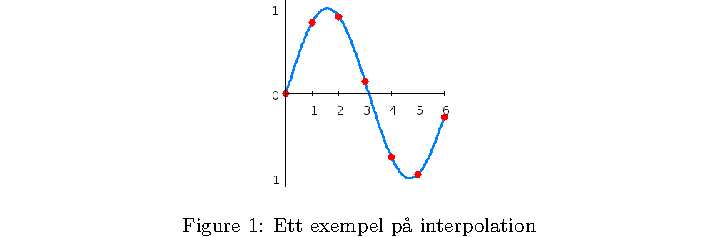
\includegraphics[width=\textwidth,clip=true,trim=80 0 80 0]{ex/4/graphicx.pdf}}
		\end{minipage}
		\caption{Koden till vänster inkluderar filen \cli{interpolation.png} i
		\LaTeX-dokumentet och ger det resultat som ses till höger.}
		\label{fig:graphicx}
	\end{figure}
	
	\subsubsection{Rätt format?}
	En nackdel med \pdfLaTeX{} när det gäller \pack{graphicx} är att det inte
	finns särskilt många bildformat som fungerar (dock fler än för gamla
	\LaTeX{}, som bara accepterade \EPS). De enda format som kan inkluderas
	med \pack{graphicx} när man använder \pdfLaTeX{} är \textsc{PNG},
	\textsc{JPEG} och \PDF. Oftast vill man använda \PDF{} för figurer,
	eftersom
	det är det enda vektorbaserade formatet som fungerar, medan man för
	fotografier och dylikt använder \textsc{JPEG}. \textsc{PNG} kan man
	använda då man egentligen bör använda \PDF{} men detta inte är möjligt.
	
	Eftersom många verktyg och programvaror fortfarande sparar filer i
	\EPS-format kan det vara praktiskt att kunna konvertera dessa till ett
	format som fungerar. Detta kan göras med verktyget \cli{epstopdf}, som
	finns tillgängligt på CTAN.
	
	\subsection{Rita med \PGFTikZ}
	Ett lite mer komplicerat sätt att inkludera grafik (men ofta 
	föredelaktigt, eftersom allt innehåll stannar i \TeX-filen) är att använda
	\PGFTikZ, ett paket skrivet för att användas med \pdfLaTeX{} för att rita
	figurer i \LaTeX{}. Med det kan man direkt i sitt \LaTeX-dokument skapa
	enklare figurer som flödesscheman, träd, grafer eller liknande; se exempel
	i figur~\vref{fig:tikz}. Även mer avancerade figurer är möjliga, men att
	förklara hela \PGFTikZ{} tar allt för lång tid för denna introduktion. Den
	intresserade läsaren hänvisas istället till \citeasnoun{Mertz07} som har
	en bra introduktion till ämnet, och \PGFTikZ-manualen \cite{Tantau10} som
	utförligt beskriver hur paketet fungerar.
	
	\begin{figure}[p]
		\centering
		\begin{minipage}{0.95\textwidth} % kod
			\vfil
			\begin{latexcode}
\newcounter{d}\setcounter{d}{0}
\def\mcolor{SpringGreen}
\begin{tikzpicture}
    \path[coordinate] (0,0)
         coordinate(A) ++( 60:6cm)
         coordinate(B) ++(-60:6cm) coordinate(C);
    \draw[fill=Black!\thed!\mcolor]
         (A) -- (B) -- (C) -- cycle;
    \foreach \x in {1,...,15}{%
        \pgfmathsetcounter{d}{\thed+10}
        \setcounter{d}{\thed}
        \path[coordinate] coordinate(X) at (A){};
        \path[coordinate] (A)
             -- (B) coordinate[pos=.15](A)
             -- (C) coordinate[pos=.15](B)
             -- (X) coordinate[pos=.15](C);
        \draw[fill=Black!\thed!\mcolor]
             (A)--(B)--(C)--cycle;
    }
\end{tikzpicture}
			\end{latexcode}
			\vfil
		\end{minipage}
		\\[1ex]
		\begin{minipage}{0.95\textwidth} % figur
			\centering
			\newcounter{density}\setcounter{density}{0}
			\begin{minipage}{0.475\textwidth}
			\fbox{\begin{tikzpicture}
			    \path[coordinate] (0,0)  coordinate(A)
			                ++( 60:0.95\textwidth) coordinate(B)
			                ++(-60:0.95\textwidth) coordinate(C);
			    \draw[fill=Black!\thedensity!SpringGreen]
							(A) -- (B) -- (C) -- cycle;
			    \foreach \x in {1,...,15}{%
			        \pgfmathsetcounter{density}{\thedensity+10}
			        \setcounter{density}{\thedensity}
			        \path[coordinate] coordinate(X) at (A){};
			        \path[coordinate] (A) -- (B) coordinate[pos=.15](A)
			                            -- (C) coordinate[pos=.15](B)
			                            -- (X) coordinate[pos=.15](C);
			        \draw[fill=Black!\thedensity!SpringGreen]
							(A)--(B)--(C)--cycle;
			    }
			\end{tikzpicture}}
			\end{minipage}\hfil
			\begin{minipage}{0.475\textwidth}
			\caption[Koden ovan tolkas av \PGFTikZ{} och resulterar i den
			itererade triangeln till vänster]{
			Koden ovan tolkas av \PGFTikZ{} och resulterar i den
			itererade triangeln till vänster.
			Fler exempel finns i
			\citeasnoun{Mertz07} och \citeasnoun{Tantau10}. Tack till Alain 
			Matthes för originalkoden\footnote{\url{http://www.texample.net/tikz/examples/rotated-triangle/}}.}
			\label{fig:tikz}
			\end{minipage}
		\end{minipage}
	\end{figure}
	
	\label{sec:4:end}
	%% (end)
	
	%% REFERENSER MED BIBTEX (fold)
	\section{Referenser med \BibTeX}\label{sec:5}
	En stor fördel med \LaTeX{} är att man kan automatisera hanteringen av
	till exempel referenser. \BibTeX{} är ett verktyg som gör detta ännu
	enklare och som gör att man kan samla alla sina referenser i en extern
	databas vilken kan hanteras av ett externt program\footnote{Exempel på
	sådana är \emph{JabRef}, \emph{BibDesk} och \emph{refbase}.\hfill} eller 
	(som sig bör när det gäller \LaTeX) med en enkel textredigerare.
	
	Systemet består av stilfiler (med filändelse \texttt{.bst}), databaser
	(\texttt{.bib}) och programmet \texttt{bibtex}. Denna introduktion kommer
	endast att gå igenom databasformatet och hur denna används från \LaTeX{}; 
	en ytterligare introduktion ges av \citeasnoun{Fenn06} och en komplett
	manual är även tillgänglig \cite{Patashnik88a}. Att skapa egna stilfiler
	involverar en del programmering i ett stackorienterat postfix-språk som
	dokumenteras av \pack{btxhak} \cite{Patashnik88b}, men detta är inte att
	rekommendera. Bättre är att använda några av de \BibTeX-stilar som finns
	på CTAN (eller \pack{chscite}%
	\footnote{\url{http://blog.sigurdhsson.org/projects/latexhax.html%
	\#chalmers-style-references-chscite}\label{fn:chscite}} om man vill följa 
	Chalmers-bibliotekets rekommendationer).
	
	\subsection{\BibTeX-databasen}
	Den databas \BibTeX{} använder är i all sin enkelhet en vanlig textfil.
	Denna textfil innehåller ett antal block, ett per referens i databasen,
	som innehåller information om referensen (\emph{fält}). En typisk referens
	innehåller en nyckel (vilken man sedan använder när man refererar till
	referensen i \LaTeX-dokumentet), en titel, en författare och ett årtal.
	Dessutom innehåller varje block information om vilken typ av referens 
	(bok, artikel och så vidare) det handlar om. 
	
	\begin{kod}[tbp]
		\centering
		\vfil\cprotect[mm]\ifdraft{\inputminted[frame=single]{latex}{ex/5/bibdata.bib}}{\inputminted[frame=single,bgcolor=mintedbg,rulecolor=\color{mintedbg}]{latex}{ex/5/bibdata.bib}}\vfil
		\caption{En enkel exempelreferens ur en \BibTeX-databas.}
		\label{ex:bibtex}
	\end{kod}
	
	Exempel~\vref{ex:bibtex} visar ett block ur en \BibTeX-databas; blocket
	inleds med en blocktyp (\texttt{@ARTICLE}) och den nyckel som används då
	man refererar till källan från \LaTeX{} (\texttt{Hassanpour08}) varefter
	ett antal självförklarande fält med information följer. Olika blocktyper
	kräver olika fält, både obligatoriska (till exempel titel och författare)
	och frivilliga (i det här fallet är bland annat \texttt{month} frivillig)
	— tabell~\vref{tab:blocktyper} listar de vanligaste blocktyperna och de
	obligatoriska/frivilliga fält som hör till.
	
	\begin{table}[bp]
		\begin{minipage}{0.98\textwidth}
			\newlength{\oldfboxsep}\setlength{\oldfboxsep}{\fboxsep}
			\setlength{\fboxsep}{0pt}
			\newcommand{\required}{% (fold)
				\setlength{\fboxsep}{\oldfboxsep}%
				\colorbox{required}{\color{required}o}%\checkmark}%
			} % (end)
			\newcommand{\optional}{% (fold)
				\setlength{\fboxsep}{\oldfboxsep}%
				\colorbox{optional}{\color{optional}v}%\Large$\circ$}%
			} % (end)
			\newcommand{\unavailable}{% (fold)
				\setlength{\fboxsep}{\oldfboxsep}%
				\colorbox{unavailable}{\color{unavailable}x}%$\times$}%
			} % (end)
			\centering
			\caption{\setlength{\oldfboxsep}{0.5\oldfboxsep}%
				Vanliga referenstyper i \BibTeX{} och deras tillhörande fält.
				Både typnamn och fältnamn är relativt självförklarande.
				\emph{Nyckel:} \fbox{\required} obligatoriskt,
				\fbox{\optional} valfritt och
				\fbox{\unavailable} otillgängligt fält.
			}
			\label{tab:blocktyper}
			\begin{tabular}{lc@{}c@{}c@{}c@{}c@{}c@{}c@{}c@{}%
							 c@{}c@{}c@{}c@{}c@{}c@{}c@{}c}
			\toprule 
			Blocktyp & % (fold)
				\rotatebox{90}{\texttt{address}} &
				\rotatebox{90}{\texttt{author}} &
				\rotatebox{90}{\texttt{booktitle}} &
				\rotatebox{90}{\texttt{chapter}} &
				\rotatebox{90}{\texttt{edition}} &
				\rotatebox{90}{\texttt{editor}} &
				\rotatebox{90}{\texttt{journal}} &
				\rotatebox{90}{\texttt{month}} &
				\rotatebox{90}{\texttt{number}} &
				\rotatebox{90}{\texttt{pages}} &
				\rotatebox{90}{\texttt{publisher}} &
				\rotatebox{90}{\texttt{school}} &
				\rotatebox{90}{\texttt{series}} &
				\rotatebox{90}{\texttt{title}} &
				\rotatebox{90}{\texttt{volume}} &
				\rotatebox{90}{\texttt{year}} \\
			% (end)
			\midrule 
			\texttt{@article} & \unavailable & \required & \unavailable & \unavailable & \unavailable & \unavailable & \required & \optional & \optional & \optional & \unavailable & \unavailable & \unavailable & \required & \optional & \required \\
			\texttt{@book}\footnote{\label{fn:auth-editor}Antingen \texttt{author} \emph{eller} \texttt{editor} ska specificeras, ej båda två.} & \optional & \required & \unavailable & \unavailable & \optional & \required & \unavailable & \optional & \unavailable & \unavailable & \required & \unavailable & \optional & \required & \optional & \required \\
			\texttt{@booklet} & \optional & \optional & \unavailable & \unavailable & \unavailable & \unavailable & \unavailable & \optional & \unavailable & \unavailable & \unavailable & \unavailable & \unavailable & \required & \unavailable & \optional \\
			\texttt{@inbook}$^\text{\ref{fn:auth-editor}}$\footnote{\label{fn:chap-pages}Det räcker med att specificera ett av fälten \texttt{chapter} och \texttt{pages}.} & \optional & \required & \unavailable & \required & \optional & \required & \unavailable & \optional & \unavailable & \required & \required & \unavailable & \optional & \required & \optional & \required \\
			\texttt{@incollection} & \optional & \required & \required & \unavailable & \unavailable & \optional & \unavailable & \optional & \unavailable & \optional & \optional & \unavailable & \unavailable & \required & \unavailable & \required \\
			\texttt{@inproceedings} & \optional & \required & \required & \unavailable & \unavailable & \optional & \unavailable & \optional & \unavailable & \optional & \optional & \unavailable & \unavailable & \required & \unavailable & \required \\
			\texttt{@manual} & \unavailable & \optional & \unavailable & \unavailable & \optional & \unavailable & \unavailable & \optional & \unavailable & \unavailable & \unavailable & \unavailable & \unavailable & \required & \unavailable & \optional \\
			\texttt{@mastersthesis} & \optional & \required & \unavailable & \unavailable & \unavailable & \unavailable & \unavailable & \optional & \unavailable & \unavailable & \unavailable & \required & \unavailable & \required & \unavailable & \required \\
			\texttt{@misc} & \unavailable & \optional & \unavailable & \unavailable & \unavailable & \unavailable & \unavailable & \optional & \unavailable & \unavailable & \unavailable & \unavailable & \unavailable & \optional & \unavailable & \optional \\
			\texttt{@phdthesis} & \optional & \required & \unavailable & \unavailable & \unavailable & \unavailable & \unavailable & \optional & \unavailable & \unavailable & \unavailable & \required & \unavailable & \required & \unavailable & \required \\
			\texttt{@proceedings} & \optional & \unavailable & \unavailable & \unavailable & \unavailable & \optional & \unavailable & \optional & \unavailable & \unavailable & \optional & \unavailable & \unavailable & \required & \unavailable & \required \\
			\texttt{@unpublished} & \unavailable & \required & \unavailable & \unavailable & \unavailable & \unavailable & \unavailable & \optional & \unavailable & \unavailable & \unavailable & \unavailable & \unavailable & \required & \unavailable & \optional \\
			\bottomrule 
			\end{tabular}
		\end{minipage}
	\end{table}
	
	Oftast är det dock lättare att hantera sin referensdatabas med någon form
	av dedikerat verktyg istället för att redigera \texttt{.bib}-filerna
	för hand med en textredigerare. Programmet JabRef%
	\footnote{\url{http://jabref.sourceforge.net/}}
	fungerar mycket bra till detta och finns tillgängligt till alla
	plattformar.
	
	Många webbaserade sökverktyg för akademiska publikationer, till exempel
	Scopus\footnote{\url{http://www.scopus.com/home.url}}, gör det möjligt att
	enkelt exportera information om de artiklar man refererar till i \BibTeX-%
	format, som sedan kan läggas till direkt i den egna referensdatabasen.
	Detta är oerhört praktiskt i större projekt, så som kandidatuppsatser.
	
	\subsection{\BibTeX{} med \LaTeX{}}
	För att referera till de referenser man har i sin referensdatabas
	i sitt \LaTeX-dokument krävs ett par olika saker. Först och främst så
	måste man specificera en bibliografistil och inkludera sin
	databas i dokumentet där man vill ha sin bibliografi:
	\begin{latexcode}
\bibliographystyle{plain}
\bibliography{databas}
	\end{latexcode}
	Notera här att bibliografistilen (mer om dessa\vpageref{sec:5:stilar})
	måste specificeras
	innan databasen inkluderas, och att databasen inkluderas med sitt namn
	\emph{utan filändelsen}; koden ovan inkluderar alltså referenser från
	filen \texttt{databas.bib}. Man kan specificera flera olika databaser
	genom att separera dem med kommatecken.
	
	När man sedan kompilerar sitt dokument måste man även köra \BibTeX{} på
	sitt dokument; detta görs genom att köra kommandot \texttt{bibtex 
	"dokument"} (om \TeX-dokumentet heter \texttt{dokument.tex}) — notera
	avsaknaden av filändelse även här. Därefter måste man köra \LaTeX{} ännu
	en gång för att referenserna ska dyka upp. En normal kompileringsrunda
	med \BibTeX{} är alltså \LaTeX$\to$\BibTeX$\to$\LaTeX$\to$\LaTeX. Med
	extra verktyg så som \texttt{latexmk} görs detta automatiskt.
	
	\BibTeX{} inkluderar dock endast de referenser som används i dokumentet
	(det vill säga sådana som refereras till direkt i texten), så om din
	referenslista inte dyker upp ska du inte vara orolig. Det finns ett antal
	olika sätt att referera till källor med \BibTeX{}; två stycken inbyggda
	(\cmd{cite} och \cmd{nocite}) samt de som definieras av olika paket (till
	exempel \pack{harvard}, vilket diskuteras~\vpageref{sec:5:harvard}).
	
	Kommandot \cmd{cite} refererar till en källa i databasen och skriver ut
	en hänvisning till bibliografin. För de ursprungliga stilarna i \BibTeX{}
	är denna hänvisning en siffra eller nyckel inom hakparanteser (alltså
	något i stil med ”[1]”), men detta kan modifieras av diverse paket och
	bibliografistilar. Kommandot tar ett obligatoriskt argument, nyckeln till
	källan i databasen, och ett frivilligt som lägger till text efter
	hänvisningen. Det frivilliga argumentet kan alltså användas för att 
	hänvisa till specifika sidor eller delar av en källa:
	\begin{latexcode}
\cite{Hassanpour08}       % Skriver ut ”[1]”
\cite[s.~5]{Hassanpour08} % Skriver ut ”[1, s. 5]”
	\end{latexcode}
	
	Notera här att det obligatoriska argumentet ska motsvara den nyckel som
	anges i databasen; här refererar vi till den källa som visas i
	exempel~\vref{ex:bibtex}.
	Man kan även referera till flera källor samtidigt genom att separera
	dessa med kommatecken:
	\latex|\cite{Hassanpour08,Khan10} % Skriver ut ”[1,2]”|
	
	Kommandot \cmd{nocite} gör samma sak som \cmd{cite} men skriver inte ut
	någon hänvisning. Detta kommando kan därför användas om man vill
	inkludera en källa i bibliografin utan att faktiskt referera till den i
	text. Här finns endast det obligatoriska argumentet. Vill man inkludera
	alla källor i databasen i sitt dokument kan man istället för en nyckel
	ange ”\texttt{*}”:
	\latex|\nocite{*}|
	
	\subsubsection{Bibliografistilar}\label{sec:5:stilar}
	Det finns en uppsjö olika sätt att referera till källor när man skriver
	vetenskapliga rapporter, och dessa kan variera kraftigt i stil. Några
	använder siffror (IEEE, Vancouver) eller nycklar (\AmS) för att hänvisa 
	till källor i text medan andra (Harvard, Chicago, APA) använder sig av
	författarnamnen.
	\BibTeX, i sitt grundutförande, kan endast skapa bibliografier och
	referenser med nycklar eller siffror. Vissa paket så som \pack{harvard}
	och \pack{chscite} implementerar dock Harvard- och Chicago-stilen.
	
	Även själva bibliografin, alltså listan över källor, kan utformas på
	oerhört många sätt. Figur~\vref{fig:bibstyle} visar några av de stilar
	som finns tillgängliga med \BibTeX{} och på CTAN. Vilken stil man vill
	använda är upp till författaren (eller kanske oftare förläggaren), men
	generellt sett så brukar man i matematiska kretsar använda 
	\texttt{alpha.bst}, i (elektro)ingenjörskretsar \texttt{ieeetr.bst} (som
	ej visas i figuren) och i humanistiska vetenskaper Harvard-stilen (eller
	någon närliggande stil). Chalmers avviker från detta och rekommenderar att
	man använder en Chicago-liknande stil~\cite{ChsLib10}.
	
	\begin{figure}[tp]
		\centering
		\subfloat[\texttt{abbrv.bst}]{\label{fig:bibstyle:abbrv}% (fold)
			\fbox{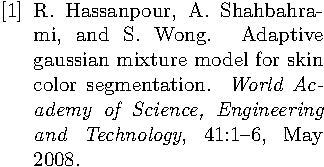
\includegraphics[width=0.45\textwidth,%
								   trim=0 -14 0 0]{ex/5/abbrv.pdf}}
		} \hfil % (end)
		\subfloat[\texttt{alpha.bst}]{% (fold)
			\fbox{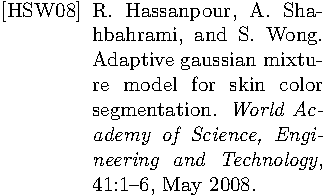
\includegraphics[width=0.45\textwidth]{ex/5/alpha.pdf}}
		} \\ % (end)
		\subfloat[\texttt{apalike.bst}]{\label{fig:bibstyle:apalike}% (fold)
			\fbox{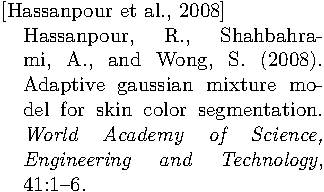
\includegraphics[width=0.45\textwidth]{ex/5/apalike.pdf}}
		} \hfil % (end)
		\subfloat[\texttt{chscite.bst} från \pack{chscite}]{% (fold)
			\label{fig:bibstyle:chscite}%
			\fbox{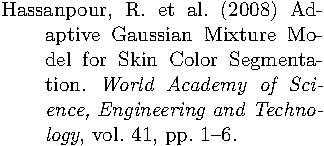
\includegraphics[width=0.45\textwidth,%
								   trim=0 -22 0 0]{ex/5/chscite.pdf}}
		} \\ % (end)
		\subfloat[\texttt{dcu.bst} från \pack{harvard}]{% (fold)
			\fbox{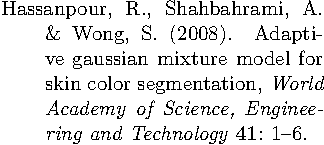
\includegraphics[width=0.45\textwidth,%
								   trim=0 -11.5 0 0]{ex/5/harvard-dcu.pdf}}
		} \hfil % (end)
		\subfloat[\texttt{jurabib.bst} från \pack{jurabib}]{% (fold)
			\label{fig:bibstyle:jurabib}%
			\fbox{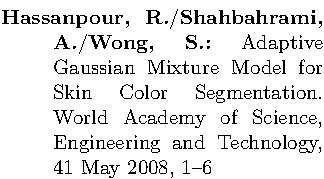
\includegraphics[width=0.45\textwidth,%
								   trim=0 0 0 5,clip=true]{ex/5/jurabib.pdf}}
		} \\ % (end)
		\caption[Några av de bibliografistilar som kan åstadkommas med
		hjälp av \BibTeX.]{Några av de bibliografistilar som kan åstadkommas
		med hjälp av \BibTeX.
		Figurerna~\subref{fig:bibstyle:abbrv}–\subref{fig:bibstyle:apalike} 
		visar standardstilar, medan  
		figurerna~\subref{fig:bibstyle:chscite}–\subref{fig:bibstyle:jurabib} 
		visar stilar som definieras av olika paket.}
		\label{fig:bibstyle}
	\end{figure}
	
	\subsubsubsection*{Harvard- och Chicago-stilen: \pack{harvard} och \pack{chscite}}\label{sec:5:harvard}
	Harvard- och Chicago-stilarna, varav den senare beskrivs utförligt i
	\emph{The Chicago Manual of Style} \cite{Chicago10},
	är sätt att referera till källor baserat
	på deras författare, och används ofta i de humanistiska vetenskaperna.
	Fördelen med dessa stilar är att referenserna smälter in bättre med den
	omgivande texten och ger ett bättre sammanhang.
	
	Tyvärr så är \BibTeX{} från början inte gjort för att stödja de här
	referensstilarna, varför det har dykt upp ett antal olika paket som
	gör det möjligt. Ett av dessa paket är \pack{harvard}, som beskrivs
	utförligt av \citeasnoun{Williams08}. Paketet definierar, förutom det
	vanliga kommandot \cmd{cite}, tre relativt självförklarande kommandon:
	\cmd{citeasnoun}, som refererar till en källa som ett substantiv,
	\cmd{possessivecite}, som refererar till en källa i genitivform,
	och \cmd{citeaffixed}, som refererar som \cmd{cite} men med ett tillägg.
	Hur dessa bör användas i text är illustreras av följande exempel:
	\begin{latexcode}
...vilket visades av \citeasnoun{Hassanpour08}.
\possessivecite{Hassanpour08} undersökning visade att...
...flera rapporter \citeaffixed{Hassanpour08}{t.ex.}...
	\end{latexcode}
		
	\label{sec:chscite}
	Även Chalmers rekommenderar att man använder en stil baserad på Chicago-%
	stilen \cite{ChsLib10}, och dessa rekommendationer implementeras av 
	paketet \pack{chscite} som bygger på \pack{harvard} och därför fungerar
	på samma sätt. Detta paket finns ännu inte på
	CTAN; se istället länken i fotnoten~\vpageref{fn:chscite}.
	%% (end)
	
	%% VIDARE LÄSNING (fold)
	\section{Vidare läsning}\label{sec:6}
	Den här introduktionen har förhoppningsvis gett dig en bra \LaTeX-grund
	som låter dig typsätta både rapporter och artiklar utan problem. Tyvärr
	kommer du, eftersom \LaTeX är ett så stort system, sannolikt att behöva
	ytterligare hjälp, tips och resurser allt eftersom du använder \LaTeX 
	och stöter på problem eller svårigheter.

	Denna del av introduktionen ämnar ge dig några tips på sådana resurser.
	Delen inleds med några relevanta resurser så som böcker och journaler
	som behandlar \TeX{} och \LaTeX på en mer eller mindre avancerad nivå,
	samt några tips när det gäller att få hjälp med specifika problem.
	Därefter följer några tips gällande stora projekt, som du sannolikt kommer
	att ha nytta av förr eller senare, speciellt om du studerar på en högskola
	eller ämnar författa böcker och liknande.

	Därefter följer en lista av viktiga och nyttiga \LaTeX-paket, som man bör
	åtminstone skumma igenom för att få en hyfsad uppfattning om vilka paket
	som finns och när man bör använda dem. Avslutningsvis ges även en lista
	över andra projekt som liknar \LaTeX, till exempel det tidigare nämnda
	\XeTeX.

	\subsection{Andra resurser}
	Även om denna introduktion siktar på att ge dig allt du behöver för att
	lära dig \LaTeX{} är det inte säkert att den är tillräcklig. Man kan inte
	diskutera allt i en kort introduktion, och vill man lära sig mer om den
	inre strukturen hos \TeX{} eller \LaTeX så finns det redan mycket bra och
	utförliga resurser tillgängliga.
	Dessutom kan man i en kort introduktion inte diskutera specifika problem
	i detalj, eftersom dessa ofta beror på den specifika situationen.

	Nedan följer därför en lista över resurser, i form av böcker, journaler
	och forum, som kan hjälpa dig släcka din kunskapstörst eller lösa dina
	\LaTeX-problem.
	
	\subsubsection{Böcker och artiklar}
	Det finns mycket material tillgängligt när det gäller \LaTeX{}. Många
	böcker inom ämnet har publicerats av Addison-Wesley, och det finns även
	en uppsjö artiklar, böcker och guider tillgängliga på CTAN, och en journal
	(\emph{The Prac\TeX{} Journal}\footnote{\url{http://tug.org/pracjourn/}})
	som finns
	tillgängliga på internet. Nedan följer en lista på några avde böcker och 
	artiklar som kan vara av intresse för dig som precis börjat med \LaTeX.
	
	\begin{description}
		\item[\emph{An essential guide to \LaTeXe{} usage} \cite{Fenn07}]
		brukar också refereras till som \pack{l2tabu} (dess namn på CTAN), och
		ger en kort lista över utdaterade paket, dödssynder inom \LaTeX{} samt
		några små tips. Förhoppningsvis lär du dig inget nytt av att läsa
		\pack{l2tabu} (det skulle ju indikera att den här introduktionen är
		felaktig), men det kan vara värt att skumma igenom den ändå.
		
		\item[\emph{The Not So Short Introduction to \LaTeXe} \cite{Oetiker11}]
		går även under namnet \pack{lshort} och är
		en kort introduktion till \LaTeX,
		skriven på engelska. Den går \emph{lite} djupare in på vissa bitar
		av \LaTeX{}, och fokuserar en del på den nu i princip överflödiga
		\LaTeX-motorn som skapar \DVI-filer, men har varit en stor inspiration
		till den här introduktionen. Absolut värd en (snabb) genomläsning.
		
		\item[\emph{Math into \LaTeX} \cite{Gratzer96}]
		ger än ännu längre introduktion till \LaTeX{} än \pack{lshort}, och
		är även den skriven på engelska. En bra ytterligare referens om det är
		något man vill veta mer om eller något man tycker är otydligt i den
		här introduktionen och \pack{lshort}.
		
		\item[\emph{Math Mode} \cite{Voss10}]
		ger en mycket ordentlig
		genomgång av matematiktypsättning både i vanliga \LaTeX{} och med
		\AmS\LaTeX{}, och är en nästintill oumbärlig referens när man skriver
		lite mer komplicerade ekvationer. Bokmärk och titta igenom varje gång
		du skriver matematik i \LaTeX.
		
		\item[\emph{Short Math Guide for \LaTeX} \cite{Downes02}]
		är en kort guide till matematik med \AmS\LaTeX{} skriven av en av
		huvudpersonerna bakom just \AmS\LaTeX. Ger några små värdefulla tips,
		en lista över symboler och en introduktion till
		\cmd{DeclareMathOperator} och några andra \AmS-konstruktioner som inte
		diskuteras utförligt i den här introduktionen. Sjutton mycket läsvärda
		sidor.
		
		\item[\emph{The \LaTeX{} Companion} \cite{Mittelbach04}]
		beskriver alla \LaTeX-kommandon och en stor mängd paket. Om du ska
		skriva ett eget paket eller en egen dokumentklass, eller bara är
		intresserad av att ”hacka” \LaTeX{} lite, så bör du absolut ta en titt
		på den här boken. En mycket bra referens för den vane \TeX{}aren.
		
		\item[\emph{\LaTeX: A Document Preparation System} \cite{Lamport94}]
		skrevs av författaren till \LaTeX{} och kan anses vara det närmsta en
		”manual” till \LaTeX{} man kan komma. Främst av historiskt intresse,
		och inget för nybörjaren.
		
		\item[\emph{\TeX{} by Topic} \cite{Eijkhout92}]
		ger en utförlig förklaring till \TeX{} och är en relevant referens för
		alla som ska utföra lågnivåarbete i \TeX{} eller \LaTeX{}. Främst
		riktad till mycket vana användare av \TeX{} och \LaTeX{}, och absolut
		inte riktad till nybörjaren.
		
		\item[\emph{The \TeX{}book} \cite{Knuth86}]
		skrevs av skaparen av \TeX{} och förklarar i detalj hur systemet
		fungerar. Främst av historiskt intresse, och egentligen bara värd att
		titta på om man vill veta hur \TeX{} \emph{egentligen} fungerar.
	\end{description}
	
	Utöver dessa bör man givetvis även läsa manualerna till de paket man
	använder (dessa finns alltid på CTAN) och kanske även manualen till
	\BibTeX{} \cite{Patashnik88a} om man behöver det.
	
	\subsubsection{Hjälp med specifika problem}
	Det tar lång tid att bemästra \LaTeX{} fullt ut, och i början kommer man
	garanterat att stöta på problem. Några av dem kanske går att lösa med den
	hjälp som ges i den här introduktionen och de andra böcker och artiklar
	som presenteras, men vissa måste man fråga någon om.
	
	Det finns så klart en uppsjö olika maillistor, forum och sökmotorer (och
	phaddrar, för dig som går på en teknisk högskola) som kan användas för att
	lösa problem, ställa frågor och utforska \LaTeX. En oerhört bra resurs är
	\emph{\TeX{} Stack Exchange}\footnote{\url{http://tex.stackexchange.com/}}
	där man kan ställa frågor om \TeX, \LaTeX{} och andra relaterade system.
	Många stora namn i \TeX-världen dyker upp där lite då och då, och undrar
	man något om \LaTeX{} så är det ett utmärkt ställe att fråga.
	
	\subsection{Tips för stora projekt}
	För stora \LaTeX{}projekt (till exempel kandidatarbeten, examensarbeten
	och liknande) är det viktigt att kunna ha en ordentlig ordning på sitt
	dokument. Är det dessutom ett dokument många ska samarbeta med är det
	ännu viktigare att det är strukturerat.
	
	Den första tumregeln, som även bör tillämpas vid mindre projekt, är att
	man bör lägga varje \LaTeX-dokument (eller projekt) i en egen undermapp.
	Ännu bättre blir det om man även lägger alla externa filer (figurer,
	inkluderad programkod och så vidare) i ännu en undermapp. En bra
	mappstruktur skulle alltså kunna se ut ungefär som i exempel
	\vref{ex:mapp}.
	
	\begin{kod}
		\begin{textcode}
.
`-- FFM233-projekt
    |-- img
    |   |-- degradering-1.png
    |   |-- degradering-2.png
    |   |-- ...
    |   |-- triangel-1.png
    |   `-- triangel-2.png
    |-- kod
    |   |-- diffekv.m
    |   |-- ode.m
    |   `-- plot.m
    |-- projekt.tex
    `-- referenser.bib
		\end{textcode}
		\caption{En bra mappstruktur för ett enkelt \LaTeX-projekt.}
		\label{ex:mapp}
	\end{kod}
	
	Utöver detta kan man se till att försöka abstrahera bort till exempel
	kommandodefinitioner eller stiländringar till ett eget paket eller en
	egen dokumentklass, om möjligt. Att göra detta lämnas som en övning åt
	läsaren, men mer information om hur man gör sådant ges av bland annat
	\citeasnoun{Flynn06}, \citeasnoun{LaTeX3} och \citeasnoun{Robertson06}.
	
	\subsubsection{Versionshantering}
	För större projekt och projekt som utförs i grupp är det mycket praktiskt
	att kunna spåra ändringar och ändra dokumentet från många olika platser
	(gärna samtidigt). Med hjälp av ett versionshanteringssystem så som 
	Git\footnote{\url{http://git-scm.com/}} eller
	Subversion\footnote{\url{http://subversion.tigris.org/}} blir detta
	enkelt. Ännu bättre blir det om man använder ett distribuerat system så
	som Mercurial\footnote{\url{http://mercurial.selenic.com/}}, hostat helt
	gratis av något snällt företag, till exempel på
	Bitbucket\footnote{\url{https://bitbucket.org/}}.
	
	Att utförligt förklara hur Mercurial fungerar är utanför den här bokens
	område, men är man intresserad bör man läsa
	\emph{Hg Init}\footnote{\url{http://hginit.com/}}, som trots sitt bruk av
	Comic Sans är en utmärkt resurs för den som vill lära sig Mercurial och
	versionshantering.
	
	\subsubsection{Uppdelning av dokumentet}
	Stora projekt (med flera kapitel eller stora delar) kan med fördel delas
	upp på flera filer. Man har då en grundfil (säg, \texttt{projekt.tex}) som
	refererar till flera olika underfiler (kanske en per kapitel, lämpligen
	placerade i en undermapp till projektet). Dessa kan man sedan inkludera
	i grundfilen på ett antal olika sätt, varpå man bara kompilerar
	
	Den första metoden för att inkludera underfilerna är \cmd{input}, som i
	princip lägger in koden från underfilen direkt där kommandot används och
	fortsätter kompilera som om koden alltid funnits där. Detta är praktiskt
	om man av någon anledning inte vill använda den andra metoden.
	
	Den andra metoden, \cmd{include}, är i princip ekvivalent till \cmd{input}
	med den skillnaden att en sidbrytning läggs in före och efter den 
	inkluderade koden. Dessutom kan man med hjälp av kommandot
	\cmd{includeonly} bestämma \emph{vilka} underfiler som inkluderas, för att
	till exempel spara tid vid kompileringen om man bara är intresserad av en
	specifik del.
	
	Den tredje och sista metoden är med paketet \pack{subfiles}. Denna är
	generellt sett att föredra om den är tillgänglig, och fungerar ungefär som
	metod ett men med undantaget att man även kan kompilera underfilerna
	var för sig, om man är intresserad av detta. Det kan vara lämpligt att
	göra om man bara redigerar ett kapitel, och inte vill kompilera hela
	projektet under tiden. Paketet \pack{subfiles} finns på CTAN men inte i
	Chalmers datorsystem eller i \TeX{} Live.
	
	\subsection{Rekommenderade paket}
	Eftersom \TeX{} är Turingkomplett kan i princip allt göras med språket,
	även om det främst är tänkt för typsättning. Således kan det mesta i 
	typsättningsväg lösas relativt enkelt. Kan det inte det, och problemet
	man vill lösa är ett relativt vanligt problem, så finns det sannolikt ett
	paket som löser problemet. Dessa paket finns listade på CTAN (se sida
	\pageref{sec:ctan}) och kan, om man använder \TeX{} Live, installeras
	med verktyget \texttt{tlmgr}.
	
	Paket i kursiv stil finns inte på Chalmers-datorer utan måste installeras
	manuellt i hemmappen. Dokumentation för alla paket finns på CTAN och kan
	även visas genom att skriva \texttt{texdoc \emph{paketnamn}} i terminalen.
	
	\subsubsection{Allmänt nyttiga paket}
	Dessa paket finns i princip alltid och tillhandahåller så grundläggande
	funktionalitet att man alltid bör använda dem. Det handlar om allt från
	tecken- och typsnittskodning till avstavning och interna länkar.
	
	\begin{description}
		\item[\pack{babel}]
		översätter interna strängar (till exempel ”Referenser” och 
		”Sammanfattning”) till det språk som önskas och gör det möjligt för
		dessa språk att avstavas ordentligt. Paketet är ett måste då man
		använder \LaTeX, men har ersatts av \pack{polyglossia} i \XeTeX.
		
		\item[\pack{fixltx2e}]
		korrigerar en del buggar i \LaTeXe-kärnan och gör till 
		exempel matematikkommandon robusta. Inkludera alltid.
		
		\item[\pack{fontenc}]
		låter användaren välja typsnittskodning. Från början använder \LaTeX{}
		\texttt{OT1}, som inte innehåller icke-anglikanska tecken så som
		\emph{å}, \emph{ä} och \emph{ö}. Detta medför problem när det gäller
		bland annat avstavning, och man bör därför istället använda 
		\texttt{T1}. Detta diskuteras närmre \vpageref{pack:fontenc}.
		
		\item[\pack{hyperref}]
		gör om innehållsförteckningar, referenser och URIer till riktiga
		länkar i de fall detta stöds (det vill säga om slutformatet är \PDF).
		Dessutom skapar den inbyggda innehållsförteckningar som kan användas
		för att navigera i dokumentet i en del \PDF-läsare (till exempel Skim
		och Acrobat Reader).
		Ett oumbärligt paket som alltid bör inkluderas.
		
		\item[\pack{inputenc}]
		är ett paket som låter användaren berätta för \LaTeX{} vilken
		teckenkodning indatan sparats med. De vanigaste inställningarna är
		\texttt{utf8} och \texttt{latin1}, men många andra teckenkodningar
		stöds också.
		Detta paket introducerades lite kort \vpageref{pack:inputenc}.
		
		\item[\pack{lmodern}]
		inkluderar typsnittet \emph{Latin Modern} för att ersätta
		\emph{Computer Modern}, standardtypsnittet i \LaTeX. Latin Modern ser
		i princip likadant ut som Computer Modern, men är skarpare och har
		fler glyfer. Det här paketet motiveras lite närmre
		\vpageref{sec:2:lmodern}.
		
		\item[\emph{\pack{nag}}]
		försöker upptäcka saker som är \emph{bad practice}, saker som kanske
		inte fungerar som man tänkt sig, och liknande. Bör inkluderas med
		alternativen \texttt{l2tabu} och \texttt{orthodox}:
		\latex|\usepackage[l2tabu,orthodox]{nag}|
	\end{description}
	
	\subsubsection{Paket för snyggare typsättning}
	Även om \LaTeX{} är mycket bra på att typsätta så blir det ibland inte
	så snyggt som man kanske kan önska. Vid dessa tillfällen kan man
	applicera diverse olika paket för att få hjälp med detta. Det gäller
	till exempel tabeller, figurtexter, SI-enheter och matematik.
	
	\begin{description}
		\item[\pack{booktabs}]
		är ett paket som gör det möjligt att skapa mycket snygga tabeller.
		Paketet diskuteras redan \vpageref{pack:booktabs}, och är i princip
		ett måste om man ska inkludera tabeller i sitt \LaTeX-dokument.
	
		\item[\pack{caption}]
		gör det möjligt att ändra stilen på figur- och tabelltexter så att de
		syns tydligare och inte smälter in i texten.
		
		\item[\emph{\pack{siunitx}}]
		gör det enklare att typsätta SI-enheter, decimaltal och vinklar på ett
		korrekt sätt för icke engelskspråkiga rapporter. Mycket användbart
		paket som tyvärr inte finns på Chalmers datorer. Förklaras lite kort
		\vpageref{sec:3:siunitx}.
	\end{description}
	
	\subsubsubsection*{Paket för matematiktypsättning}
	Som teknisk matematiker (eller fysiker) kommer stora delar av de rapporter
	man skriver oundvikligen innehålla matematik. Även om \LaTeX{} för sig
	självt är relativt bra på att typsätta matematik kan det ibland behövas
	några tillägg för att göra det enklare. Många av dessa tillhandahålls av
	\AmS{} i det som kallas \AmS\LaTeX, men det finns fler relevanta
	matematikpaket.
	
	\begin{description}
		\item[\pack{amscd}]
		ger möjlighet att skapa kommutationsdiagram med \LaTeX:
		\begin{equation*}
			\begin{CD}
				\cov(\mathcal{L}) @>>> \non(\mathcal{K}) @>>> \cf(\mathcal{K}) @>>> \cf(\mathcal{L})\\
				@VVV @AAA @AAA @VVV\\
				\add(\mathcal{L}) @>>> \add(\mathcal{K}) @>>> \cov(\mathcal{K}) @>>> \non(\mathcal{L})
			\end{CD}
		\end{equation*}
		
		\item[\pack{amsmath}]
		gås igenom av del~\ref{sec:3} och är i princip oumbärligt om man ska
		typsätta matematik med \LaTeX. Inkludera alltid detta paket om du
		skriver något som kan tänkas innefatta ekvationer.
	
		\item[\pack{amssymb}]
		definierar en hel del matematiska symboler, till exempel 
		\cmd{therefore} (\(\therefore\)) och \cmd{ggg} (\(\ggg\)), och 
		kommandot \cmd{mathbb} som ger krittavletecken (som
		används för de grundläggande talmängderna).
		
		\item[\pack{amsthm}]
		definierar omgivningar för att typsätta teorem, satser, lemman, bevis
		och dylikt. Användbart i vissa sammanhang, främst för att typsätta
		föreläsningsanteckningar eller uppgifter. 
		
		\item[\pack{mathtools}]
		lagar några småfel i \pack{amsmath} och definierar kommandon som till
		exempel \cmd{DeclarePairedDelimiter}, som introducerades
		\vpageref{cmd:declarepaireddelimiter}.
	\end{description}
	
	\subsubsection{Paket för grafik}
	Grafik i form av figurer eller illustrationer är givetvis en viktig del
	av många rapporter, vare sig det är figurer av uppställningar, plottar
	eller flödesscheman. Det finns tre relevanta paket när det gäller grafik
	i \LaTeX; ett som används för att importera grafik från externa filer och
	två som används för att rita direkt med \LaTeX-kommandon.
	
	\begin{description}
		\item[\pack{graphicx}]
		förklaras kort i del \vref{sec:4} och gör det möjligt att inkludera
		figurer från externa filer i sitt \LaTeX-dokument. Mycket användbart
		om man har data från till exempel MATLAB eller Mathematica.
		
		\item[\pack{tikz}]
		nämns också i del \ref{sec:4} och gör det möjligt att rita
		vektorbaserade figurer direkt i \LaTeX. Mycket användbart om man
		vill rita exempelvis uppställningar, enklare illustrationer eller 
		flödesscheman, men kan användas till otroligt mycket mer. Fungerar
		endast med \pdfLaTeX{} i \PDF-läge eller moderna varianter som
		\XeTeX.
	
		\item[\pack{pstricks}]
		är en slags motsvarighet till \pack{tikz} som endast fungerar med de
		\LaTeX-varianter som genererar \DVI- eller \textsc{PS}-filer. Inte
		lika användbart som \pack{tikz} eftersom det inte fungerar med 
		\pdfLaTeX{} i \PDF-läge.
	\end{description}
	
	\subsubsection{Paket för bibliografier}
	Även om \BibTeX ofta är tillräckligt för att kunna typsätta dokument som
	ska skickas till journaler eller förläggare (eftersom verktyget
	inkluderar många vanliga engelskspråkiga bibliografistilar) så är det inte
	alltid tillräckligt. Till exempel så rekommenderar Chalmers bibliotek
	en bibliografistil som inte finns med i \BibTeX och som till råga på allt
	ska vara på svenska. Sådana problem löses enkelt av diverse paket.
	
	\begin{description}
		\item[\emph{\pack{chscite}}]
		är ett paket som skapats för att implementera de rekommendationer
		Chalmers Bibliotek publicerat \cite{ChsLib10} i \BibTeX.
		Rekommenderas absolut för alla sorters rapporter, artiklar och
		publikationer du kan tänkas producera under din studietid, så länge
		det inte finns krav på stil från annat håll. Diskuteras även
		\vpageref{sec:chscite}.
	\end{description}
	
	\subsubsection{Paket som löser problem}
	Ibland vill man göra något som är väldigt svårt att göra med vanlig
	\LaTeX-kod, till exempel ändra sidstorlek eller skapa underfigurer. Då
	många sådana problem är vanligt förekommande finns det ofta paket som
	löser dem.
	
	\begin{description}
		\item[\pack{float}]
		definierar ett kommando \cmd{newfloat} som skapar nya sorters flytande
		objekt (vilka diskuterats \vpageref{sec:floats}).
		
		\item[\pack{geometry}]
		kan användas för att ändra en del mått i \LaTeX (till exempel sidans
		storlek eller marginalerna) om så önskas. Oftast behöver man inte göra
		detta, eftersom dokumentklassen har definierat de mått den har av en
		anledning. Kan vara värdefullt om man vill skapa dokument för A5-%
		eller A6-papper (eller andra ovanliga storlekar).
	
		\item[\pack{multirow}]
		gör det möjligt att i tabeller skapa celler som spänner över flera
		rader.
		
		\item[\pack{sidecap}]
		definierar omgivningen \env{SCfigure} som typsätter en figur med
		figurtexten brevid istället för under eller över figuren. Kan vara
		användbart om man har smala figurer med lång figurtext.
		
		\item[\pack{subfig}]
		definierar kommandon som möjliggör skapandet av ”underfigurer”, det
		vill säga grupper av relaterade figurer som alla kan refereras till
		antingen som grupp (till exempel ”Figur 1”) eller individuellt (till
		exempel ”Figur 1a”).
		
		\item[\pack{varioref}]
		gör det möjligt att, med hjälp av kommandot \cmd{vref},
		skapa korsreferenser (se \vpageref{sec:labels})
		som inte bara refererar till etiketterna med nummer utan även till den
		sida figuren eller tabellen finns på. Detta görs på ett intelligent
		sätt, så att referensen blir ”figur X på nästa sida” om figuren är på
		nästa sida, och så vidare. Mycket relevant paket, speciellt i större
		rapporter.
		
		\item[\pack{wrapfig}]
		skapar ett nytt flytande objekt \texttt{wrapfig} som placerar figuren
		till höger eller vänster på sidan och låter övrig text ”flyta” runt
		figuren.
	\end{description}
	
	\subsubsection{Paket för att ändra utseende}
	Standardklasserna lämnar ofta en del att önska i termer av utseende. Vill
	man göra något åt detta kan man använda paket som utformats för att låta
	dig ändra stilen av vissa element, till exempel rubriker eller sidhuvuden.
	
	\begin{description}
		\item[\pack{fancyhdr}]
		låter dig förändra sidhuvud och sidfot för att införa snyggare, mer
		informativa eller tydligare stilar. Till exempel så kan texten i
		sidhuvudet ändras för att visa sidnummer och kapitel, medan sidfoten
		ändras för att visa till exempel kontakt- eller copyrightinformation.
		
		\item[\pack{titlesec}]
		gör det möjligt att ändra stilen på rubrikerna i dokumentet, till
		exempel genom att byta textstil eller sättet rubriken typsätts.
	
		\item[\pack{tocloft}]
		definierar kommandon för att styra utseendet av
		innehållsförteckningen.
	\end{description}
	
	\subsubsection{Andra specialiserade paket}
	För en del snäva områden så som kvantfysik eller datavetenskap, finns det
	specialiserade paket som löser specifika uppgifter. Dessa kan med fördel
	användas om man skriver rapporter inom området, eller rör vid ämnet i
	någon inlämningsuppgift.
	
	\begin{description}
		\item[\pack{algorithmic}]
		är ett paket för typsättning av algoritmer och pseudokod.
		
		\item[\emph{\pack{braket}}]
		definierar kommandon för att handskas med braket-notationen som
		används inom kvantfysik. Kommandot \cmd{Braket} kan således resultera
		i följande ekvation:
		\begin{equation*}
			\Braket{\phi|\dfrac{\partial^2}{\partial t^2}|\psi}
		\end{equation*}
		
		Paketet definierar även kommandot \cmd{Set}, för att på liknande
		sätt typsätta mängddefinitioner:
		\begin{equation*}
			\Set{x\in\mathbf{R}^2|0<{|x|}<5}
		\end{equation*}
		
		\item[\pack{listings}]
		kan användas för att inkludera programkod i \LaTeX-dokument. Det finns
		möjlighet att skriva ut radnummer, lägga till ramar, associera
		figurtexter och även en mycket enkel syntaxfärgning \eng{syntax
		highlighting}. Fungerar inte om koden innehåller svenska tecken, även
		om paketet \emph{\pack{listingsutf8}} försöker lösa detta. Använder 
		man \XeTeX uppstår inte detta problem.
		
		\item[\emph{\pack{minted}}]
		kan sägas vara en förbättring av \pack{listings} som använder Python-%
		programmet \emph{Pygments} för att även sätta färg på koden. Ett bra
		alternativ om man ska inkludera kod och vill ha fullständig
		syntaxfärgning. Paketet lider dock av samma problem med svenska tecken
		som \pack{listings}.
	\end{description}
	
	\subsection{Andra \TeX-baserade projekt}
	\LaTeX{} är inte det enda användbara \TeX-baserade projektet, även om det
	är det makropaket som används mest i praktiken. Det finns alternativ
	som baseras på \LaTeX{} men löser problem (till exempel \XeTeX och
	\hologo{LuaTeX}) men även alternativa makropaket som är mycket olika
	\LaTeX{} i sin struktur (till exempel \hologo{ConTeXt}). Dessutom finns
	det projekt för att utveckla \LaTeXe{} och göra vissa saker som till 
	exempel utveckling av dokumentklasser mycket enklare.
	
	\subsubsection{Unicode-baserade \XeTeX}
	\XeTeX är, precis som \pdfLaTeX, en \TeX-kompilator. Denna kan användas
	på samma sätt som vanliga \TeX{} och \pdfLaTeX (dvs. den kan köras på i
	princip samma kod) med hjälp av dess program, \texttt{xelatex}.
	
	Skillnaden mellan \pdfLaTeX{} och \XeTeX som gör att man kanske föredrar
	det senare är relativt stor, sett till de djupa delarna av \TeX: \XeTeX 
	förutsätter, till skillnad från \pdfLaTeX, att all indata är \UTF och kan
	därmed läsa \UTF-dokument på ett korrekt sätt. Detta innebär bland annat
	att saker som inte fungerar i \pdfLaTeX, även med \pack{inputenc}, till
	exempel svenska tecken i kodlistingar eller inkluderade filer kommer att
	fungera utmärkt med \XeTeX.
	
	Dessutom kan man med hjälp av speciella kommandon välja typsnitt på ett
	mycket enklare sätt, eftersom \XeTeX stödjer \textsc{OTF}- och
	\textsc{TTF}-typsnitt, och kan hitta alla typsnitt som är installerade
	på datorn, inte bara de som finns i form av \LaTeX-paket.
	
	En relativt övergripande bild av vad som är nytt i \XeTeX ges av
	\citeasnoun{Robertson11}; för det mesta kan man förutsätta att \LaTeX-kod
	kommer att fungera precis likadant i \XeTeX.
	
	\subsubsection{Skripta med \hologo{LuaTeX}}
	\Hologo{LuaTeX} är en kombination av programmeringsspråket Lua och
	typsättningsspråket \TeX. Introduktionen till \hologo{LuaLaTeX},
	som är \hologo{LuaTeX}s motsvarighet till vanliga \LaTeX,
	beskriver systemet som uppföljaren till \pdfLaTeX:
	\begin{quote}
		\begin{english}
			It is the designated successor of pdf\TeX{} and includes all of 
			its core features: direct generation of \PDF files with support 
			for advanced \PDF features and micro-typographic enhancements to 
			\TeX{} typographic algorithms.
			
			\hfill\cite{Gonnard10}\hspace{-1ex}%
		\end{english}
	\end{quote}
	
	I många avseenden är \hologo{LuaTeX} mycket likt \XeTeX; man kan använda
	konventionella typsnitt med båda motorerna (med paketet \pack{fontspec}), 
	och de hanterar båda \UTF 
	mycket bättre än sina företrädare. Skillnaden är att \hologo{LuaTeX}
	även gör det möjligt att bädda in Lua-kod direkt i dokumentet, vilket gör
	en del saker mycket enklare eftersom man har tillgång till ett fullgott
	skriptspråk.
	
	\subsubsection{Ett alternativ: \hologo{ConTeXt}}
	\Hologo{ConTeXt} är ett alternativt makropaket för \TeX{} som utvecklats
	parallellt med \LaTeX{} men med en annan inriktning. Medan \LaTeX{}
	försöker isolera användaren från typografiska beslut, vilket gör det
	lämpligt för att till exempel skicka in artiklar till förlag, så
	försöker \hologo{ConTeXt} ge användaren en lite mer strukturerad tillgång
	till de typografiska funktionerna i \TeX.
	
	Det finns en del artiklar som jämför \hologo{ConTeXt} och \LaTeX{}
	\citeaffixed{Hoekwater98}{till exempel}, men kontentan av det hela är att
	\LaTeX{} är vanligare i akademiska kretsar och bättre på att typsätta
	matematik, och att man därför oftast bör hålla sig till \LaTeX. Är man
	trots detta intresserad av \hologo{ConTeXt} bör man referera till
	\hologo{ConTeXt}-manualen \cite{Hagen01}.
	
	%\subsubsection{Framtiden: \LaTeX3}
	%\cite{Rowley99}
	
	%% (end)
	
	%% BIBLIOGRAFI/REFERENSLISTA (fold)
	\begin{english}
		\renewcommand\refname{Referenser}
		\let\oldurl=\url\renewcommand\url[1]{\newline{\small\oldurl{#1}}}
		\cleardoublepage
		\addcontentsline{toc}{section}{\hspace{1.3em}Referenser}
		\bibliography{referenser}
	\end{english}
	%% (end)
	
	\appendix
	%% EN ENKEL MALL (fold)
	\section{En enkel mall}\label{app:1}
	Följande mall är tänkt att användas för att skriva enklare rapporter på
	Chalmers Tekniska Högskola. Eftersom \LaTeX-installationen på deras
	datorer saknar en del paket (\pack{siunitx} och \pack{chscite}) är dessa
	bortkommenterade. Vill man ändå använda dem kan man installera dessa i
	sin hemmapp, under \texttt{\textasciitilde/texmf/}%
	\footnote{Detta förklaras närmre av \citeasnoun[ss.~89–90]{Oetiker11}%
	\hfill}.
	
	Kommentarerna och texten i mallen bör förklara och motivera vad som görs
	vilka paket som inkluderas någorlunda. Om något är oklart, referera till
	motsvarande del av den här introduktionen. Hela mallen finns dessutom
	tillgänglig som en \texttt{.tex}-fil för nedladdning%
	\footnote{\url{http://blog.sigurdhsson.org/projects/latexbok.html}}.
	
	\ifdraft{\inputminted[frame=single]{latex}{ex/A/mall.tex}}{\inputminted[frame=single,bgcolor=mintedbg,rulecolor=\color{mintedbg}]{latex}{ex/A/mall.tex}}
	%% (end)

	\backmatter
	\pagestyle{empty}
	\cleardoublepage\hbox{}\newpage
	{ % EXTERNAL BACK PAGE (fold)
		\pagecolor{\frontpagecolor}
		\color{White}
		\frontpagegraphic
		\begin{tikzpicture}[remember picture,overlay]
			\node [anchor=south east,above=2cm,right=-3.75cm] at (current page.south east)
			 			{
\includegraphics[width=3cm]{qrcode.pdf}};
		\end{tikzpicture}
		\normalcolor
		\newpage
		\pagecolor{White}
	} % (end)
\end{document}